% This is part of Un soupçon de mathématique sans être agressif pour autant
% Copyright (c) 2012
%   Laurent Claessens
% See the file fdl-1.3.txt for copying conditions.


% This is part of Un soupçon de mathématique sans être agressif pour autant
% Copyright (c) 2012-2013
%   Laurent Claessens
% See the file fdl-1.3.txt for copying conditions.


\usepackage{etex}
\usepackage{ifthen}
%\usepackage{pdfsync}       % This package is obsolete : compile with pdflatex -synctex=1 instead.

\usepackage{latexsym}
\usepackage{amsfonts}
\usepackage{amsmath}
\usepackage{amsthm}
\usepackage{amssymb}
\usepackage{bbm}
\usepackage{mathrsfs}           
\usepackage{mathabx}           % Pour \divides

\usepackage{framed}

\usepackage{calc}   % Les dépendances de phystricks si on n'utilise que le pdf.
%\usepackage{pstricks,pst-eucl,pstricks-add,calc,pst-math}   % Les dépendances de phystricks. Peut être qu'il faut ajouter catchfile
\usepackage{graphicx}                   % Pour l'inclusion d'image en pfd.

\newcommand{\EpsOrPdfincludegraphics}[2][]{%
        \ifpdf
            \includegraphics[#1]{#2.png}
        \else
            \includegraphics[#1]{#2.eps}
        \fi
        }

\usepackage{subfigure}

\usepackage{fancyvrb}
\usepackage{stmaryrd}       % Pour le \obslash
\usepackage{xstring}        % Utilisé pour les références vers wikipédia
\usepackage{cases}
\usepackage{lscape}         % pour l'environnement landscape, utilisé dans la correction corr0076.tex
\usepackage{multicol}
\usepackage{import}         % Pour le hack qui sert à inclure GeomAnal

% TODO : n'en utiliser qu'un
\usepackage[normalem]{ulem}		% Pour le barré, commande \sout
\usepackage{soul}		% Pour le barré, commande \st

\usepackage[all]{xy}

\let\second\undefined      % le paquet amthabx définit \second
\let\degree\undefined       % le paquet amthabx définit \degree
\usepackage[cdot,thinqspace,amssymb]{SIunits} 
 % L'option amssymb sert à éviter un conflit avec la commande \square de amssymb. Note qu'elle n'est plus accessible. Si tu en as besoin, faudra RTFM
%ftp://ftp.belnet.be/packages/ctan/macros/latex/contrib/SIunits/SIunits.pdf

\usepackage[nottoc]{tocbibind}

%%%%%%%%%%%%%%%%%%%%%%%%%%
%
%   Trucs mathématiques
%
%%%%%%%%%%%%%%%%%%%%%%%%

% ENSEMBLES DE NOMBRES
\newcommand{\eA}{\mathbbm{A}}
\newcommand{\eC}{\mathbbm{C}}
\newcommand{\eD}{\mathbbm{D}}
\newcommand{\eE}{\mathbbm{E}}
\newcommand{\eF}{\mathbbm{F}}
\newcommand{\eG}{\mathbbm{G}}
\newcommand{\eH}{\mathbbm{H}}
\newcommand{\eK}{\mathbbm{K}}
\newcommand{\eL}{\mathbbm{L}}
\newcommand{\eM}{\mathbbm{M}}
\newcommand{\eN}{\mathbbm{N}}
\newcommand{\eP}{\mathbbm{P}}
\newcommand{\eQ}{\mathbbm{Q}}
\newcommand{\eR}{\mathbbm{R}}
\newcommand{\eZ}{\mathbbm{Z}}

% ENSEMBLES de fonctions
\newcommand{\aL}{\mathcal{L}}       % Les applications linéaires
\newcommand{\aC}{\mathcal{C}}       % Les fonctions C^1, C^2 etc

% AUTRES
\newcommand{\sdS}{\mathcal{S}}      % L'ensemble des subdivisions d'un intervalle.



\newcommand{\mF}{\mathcal{F}}
\newcommand{\mC}{\mathcal{C}}
\newcommand{\mG}{\mathcal{G}}
\newcommand{\mI}{\mathcal{I}}
\newcommand{\mL}{\mathcal{L}}
\newcommand{\mS}{\mathcal{S}}   % Utilisé pour l'espace des fonctions Schwartz
\newcommand{\mZ}{\mathcal{Z}}


\newcommand{\mtu}{\mathbbm{1}}              % La matrice unité
\newcommand{\caract}{\mathbbm{1}}    % Characteristic function of a set

\DeclareMathOperator{\val}{val}     % valuation d'un polynôme


%\newcommand{\efrac}[2]{\frac{ \displaystyle #1 }{\displaystyle #2 }}
%%%%%%%%%%%%%%%%%%%%%%%%%%
%
%   Numérotations en tout genre
%
%%%%%%%%%%%%%%%%%%%%%%%%

\setcounter{tocdepth}{2}        % Profondeur de la table des matières
\setcounter{secnumdepth}{2}     % Profondeur dans le texte

%%%%%%%%%%%%%%%%%%%%%%%%%%
%
%   Les lignes magiques pour le texte en français.
%
%%%%%%%%%%%%%%%%%%%%%%%%

\usepackage[utf8]{inputenc}
\usepackage[T1]{fontenc}

\usepackage{listingsutf8}
\lstset{language=python,basicstyle=\footnotesize,tabsize=3,numbers=left,numberstyle=\tiny,frame=single,commentstyle=\ttfamily\color[rgb]{0,0,0.5},stringstyle=\color[rgb]{0,0.5,0},title=\lstname,inputencoding=utf8/latin1}

\usepackage[fr]{exocorr}
\usepackage{textcomp}
\usepackage{lmodern}
\usepackage[a4paper,margin=2cm]{geometry} 
\usepackage[english,frenchb]{babel}


\usepackage{hyperref}                           %Doit être appelé en dernier.
\hypersetup{
colorlinks=true,
linkcolor=blue,
urlcolor=magenta,     % couleur des url
filecolor=magenta   % couleur des textes qui sont des liens
}

%%%%%%%%%%%%%%%%%%%%%%%%%%
%
%   Les théorèmes et choses attenantes
%
%%%%%%%%%%%%%%%%%%%%%%%%


\newcounter{numtho}
\newcounter{numprob}

\makeatletter
\@addtoreset{numtho}{chapter}
%\@addtoreset{CountExercice}{chapter}
\@addtoreset{chapter}{part}
\makeatother

\newlength{\EnvSpace}
\setlength{\EnvSpace}{9pt}      % C'est la distance que je veux mettre avant et après les théorèmes, remarques, etc.

\newtheoremstyle{MyTheorems}%
        {\EnvSpace}{\EnvSpace}%
        {\itshape}%
        {}%
        {\bfseries}{.}%
        {\newline}%
        {}%
\newtheoremstyle{MyExamples}%
        {\EnvSpace}{\EnvSpace}%
        {}%
        {}%
        {\bfseries}{.}%
        {\newline}%
        {}%
\newtheoremstyle{MyRemarks}%
        {\EnvSpace}{\EnvSpace}%
        {}%
        {}%
        {\bfseries}{.}%
        {\newline}%
        {}%

%\theoremstyle{MyExamples}   %\newtheorem{exemple}[numtho]{Exemple}      % Pour unification, ne plus utiliser
%                            \newtheorem{example}[numtho]{Exemple}
\newcounter{CounterExample}
\renewcommand{\theCounterExample}{\thechapter.\arabic{CounterExample}}

\newenvironment{example}{\vspace{\EnvSpace}\refstepcounter{numtho}\noindent{\bf Exemple \thenumtho}\newline}{\phantom{a}\hfill $\triangle$\vspace{\EnvSpace}}
\newenvironment{Aretenir}{\refstepcounter{numtho}\begin{oframed}\noindent{\bf À retenir \thenumtho}\newline}{\end{oframed}\vspace{\EnvSpace}}
\newenvironment{Enmini}{\begin{oframed}\noindent{\bf Mini résumé}\newline}{\end{oframed}\vspace{\EnvSpace}}
\newenvironment{definition}{\refstepcounter{numtho}\begin{oframed}\noindent{\bf Définition \thenumtho}\newline}{\end{oframed}\vspace{\EnvSpace}}
\newenvironment{propriete}{\refstepcounter{numtho}\begin{oframed}\noindent{\bf Propriété \thenumtho}\newline}{\end{oframed}\vspace{\EnvSpace}}

\theoremstyle{MyRemarks}    \newtheorem{remark}[numtho]{Remarque}

                \newtheorem{amusement}[numtho]{Amusement}
                \newtheorem{erreur}[numtho]{Error}
                \newtheorem{probleme}[numprob]{\fbox{\bf Problèmes et choses à faire}}


\theoremstyle{MyTheorems}
            \newtheorem{lemma}[numtho]{Lemme}
            \newtheorem{corollary}[numtho]{Corollaire}
            \newtheorem{theorem}[numtho]{Théorème}      
            \newtheorem{proposition}[numtho]{Proposition}      

            %\newtheorem{exo}[CountExercice]{Exercice}       % C'est provisoire, pour Chafaï

\renewcommand{\thenumtho}{\thechapter.\arabic{numtho}}
% La numérotation des équations change dans les corrigés
\renewcommand{\theequation}{\thechapter.\arabic{equation}}
\renewcommand{\theCountExercice}{\arabic{CountExercice}}       % Ce compteur est défini dans SystemeCorr.sty
\newcommand{\defe}[2]{\textbf{#1}\index{#2}}

\renewcommand{\labelenumi}{\theenumi}
\renewcommand{\theenumi}{(\arabic{enumi})}


%%%%%%%%%%%%%%%%%%%%%%%%%%
%
%   Les macros qui font des choses
%
%%%%%%%%%%%%%%%%%%%%%%%%

\newcommand{\mA}{\mathcal{A}}
\newcommand{\mO}{\mathcal{O}}
\newcommand{\mR}{\mathcal{R}}
\newcommand{\mT}{\mathcal{T}}
\newcommand{\mU}{\mathcal{U}}

\newcommand{\scal}[2]{ \langle #1,#2\rangle }

\newcommand{\tq}{\text{ tel que }}
\newcommand{\tqs}{\text{ tels que }}
\newcommand{\quext}[1]{ \footnote{\textsf{#1}}  }
\newcommand{\info}[1]{\texttt{#1}}
\newcommand{\vect}[1]{\overrightarrow{#1}}    % Cette macro est codée en dur dans phystricksDefVecteurAXDDGP et dans d'autres

\newcommand{\VarAbs}{\text{Var}_{\text{abs}}}
\newcommand{\VarRel}{\text{Var}_{\text{rel}}}

\newcommand{\normal}{\lhd}
\newcommand{\swS}{\mathscr{S}}          % L'ensemble des fonctions Schwartz

%\newcommand{\defD}{\mathscr{D}}     % Ensemble de définition d'une fonction
\newcommand{\defD}{D}                % Le D avec des croles était impossible à comprendre pour les élèves.

\newcommand{\Borelien}{\mathcal{B}\text{or}}       % Les boréliens
\newcommand{\tribA}{\mathcal{A}}            % Une tribu A
\newcommand{\tribB}{\mathcal{B}}            
\newcommand{\tribF}{\mathcal{F}}            % Une tribu F

\newcommand{\affE}{\mathcal{E}}            % Un espace affine E
\newcommand{\affF}{\mathcal{F}}            
\newcommand{\affG}{\mathcal{G}}            

\newcommand{\statS}{\mathcal{S}}            % Un modèle statistique
\newcommand{\partP}{\mathcal{P}}            % L'ensemble des parties d'un ensemble

\newcommand{\polyP}{\mathcal{P}}            % L'ensemble des polynômes

\newcommand{\dB}{\mathscr{B}}       % la distribution de Bernoulli
\newcommand{\dE}{\mathscr{E}}       % la distribution exponentielle
\newcommand{\dG}{\mathscr{G}}       % la distribution géométrique.
\newcommand{\dM}{\mathscr{M}}       % la distribution multinomiale
\newcommand{\dN}{\mathscr{N}}       % la distribution normale.
\newcommand{\dP}{\mathscr{P}}       % la distribution de Poisson.
\newcommand{\dT}{\mathscr{T}}       % la distribution de Student
\newcommand{\dU}{\mathscr{U}}       % la distribution uniforme

\newcommand{\hL}{\mathscr{L}}       
\newcommand{\cL}{\hL}           % Pour la partie Chafai

\newcommand{\modE}{\mathcal{E}}         % Le E des modules
\newcommand{\modF}{\mathcal{F}}         % Le F des modules
\newcommand{\hH}{\mathscr{H}}           % Le H des espaces de Hilbert

%%%%%%%%%%%%%%%%%%%%%%%%%%
%
%   Bibliographie, index et liste des notations
%
%%%%%%%%%%%%%%%%%%%%%%%%

\usepackage{makeidx}
\usepackage[nottoc]{tocbibind}      % Le paquetage qui fait en sorte que la biblio soit inclue correctement dans la table des matières.
\usepackage[refpage]{nomencl}
\renewcommand{\nomname}{Liste des notations}
%
%   Comment introduire des éléments dans l'index des notations.
%
% La liste des tags à mettre pour bien classer mes notations est :
% T     pour la topologie et théorie des ensembles
%
% La syntaxe est facile, par exemple 
%       $\SL(2,\eR)$\nomenclature[G]{$\SL(2,\eR)$}{Le groupe de matrices deux par deux de déterminant 1.}
%\renewcommand{\nomgroup}[1]{%
%    \ifthenelse{\equal{#1}{A}}{\item[\textbf{Algèbre}]}{}%
%    \ifthenelse{\equal{#1}{G}}{\item[\textbf{Géométrie}]}{}%
%    \ifthenelse{\equal{#1}{R}}{\item[\textbf{Théorie des groupes}]}{}%
%    \ifthenelse{\equal{#1}{P}}{\item[\textbf{Probabilités et statistique}]}{}%
%    \ifthenelse{\equal{#1}{Y}}{\item[\textbf{Analyse}]}{}%
%    \ifthenelse{\equal{#1}{M}}{\item[\textbf{Chaînes de Markov}]}{}%
%}

%%%%%%%%%%%%%%%%%%%%%%%%%%
%
%   DeclareMathOperator
%
%%%%%%%%%%%%%%%%%%%%%%%%

\DeclareMathOperator{\signe}{sgn}
\DeclareMathOperator{\Vol}{Vol}
\DeclareMathOperator{\Int}{Int}     % Intérieur d'un ensemble.
\DeclareMathOperator{\Ind}{Ind}     % l'indice d'un chemin en analyse complexe
\DeclareMathOperator{\Diam}{Diam}   
\DeclareMathOperator{\id}{Id}   
\DeclareMathOperator{\Graph}{Graph} 
\DeclareMathOperator{\pr}{\texttt{proj}}
\DeclareMathOperator{\dom}{dom}

\DeclareMathOperator{\Graphe}{Gr}
\DeclareMathOperator{\Spec}{Spec}   % spectre d'un opérateur
\DeclareMathOperator{\arctg}{arctg}
\DeclareMathOperator{\cotg}{cotg}
\DeclareMathOperator{\cosec}{cosec}
\DeclareMathOperator{\arcsinh}{arcsinh}

\DeclareMathOperator{\GL}{GL}   % le groupe linéaire
\DeclareMathOperator{\PGL}{PGL}   % le groupe projectif
\DeclareMathOperator{\SO}{SO}           
\DeclareMathOperator{\SL}{SL}           
\DeclareMathOperator{\PSL}{PSL}   % Le groupe modulaire SL(2,Z)/Z2
\DeclareMathOperator{\gO}{O}           
\DeclareMathOperator{\SU}{SU}           
\DeclareMathOperator{\gU}{U}           

\DeclareMathOperator{\Reel}{Re}        % La partie réelle d'un nombre complexe

\DeclareMathOperator{\Image}{Image}        % ... avec \Image qui donne l'image d'une fonction ou d'un opérateur.
\DeclareMathOperator{\rang}{rg}   
\DeclareMathOperator{\Kernel}{Ker}
\DeclareMathOperator{\Domaine}{Dom}
\DeclareMathOperator{\Span}{Span}
\DeclareMathOperator{\Hom}{Hom}
\DeclareMathOperator{\End}{End}     % L'ensemble des endomorphismes
\DeclareMathOperator{\tr}{Tr}       % la trace
\DeclareMathOperator{\Majorant}{Maj}
\DeclareMathOperator{\codim}{codim} % pour la codimension.
\DeclareMathOperator{\diam}{diam} % le diamètre d'un ensemble.

\DeclareMathOperator{\Var}{Var}     % Variance d'une variable aléatoire.
\DeclareMathOperator{\Fun}{\texttt{Fun}}     % Ensemble des applications d'un ensemble vers l'autre.
\DeclareMathOperator{\Cov}{Cov}     % la covariance.
\DeclareMathOperator{\gr}{gr}     % le groupe engendré
\DeclareMathOperator{\pgcd}{pgcd}     
\DeclareMathOperator{\ppcm}{ppcm}     
\DeclareMathOperator{\Frob}{Frob}     
\DeclareMathOperator{\Card}{Card}       % Le cardinal d'un ensemble.
\DeclareMathOperator{\Stab}{Stab}       % Le stabilisateur d'un point sous l'action d'un groupe.

\DeclareMathOperator{\Frac}{Frac}       % le corps des fractions d'un anneau
\DeclareMathOperator{\Aff}{Aff}         %  l'espace affine engendré

\newenvironment{subproof}{\begin{description}}{\end{description}}

%%%%%%%%%%%%% TRUCS DE YVIK POUR FAIRE FONCTIONNER CdI1 %%%%%%%%%%%%%%%%%%%%%%
%

%\newcommand{\proofend}{\hspace*{\fill} $\Box$\\}
%\newcommand{\diam}{\hspace*{\fill} $\Diamond$\\}
%\def\s{\smallskip}
%\def\m{\medskip}
%\def\my{\bf}
\newcommand{\eps}{\varepsilon}
\newcommand{\Ker}{\operatorname{Ker}}
\newcommand{\IM}{\operatorname {Im}}
\newcommand{\cat}{\operatorname{cat}}
\newcommand{\crit}{\operatorname{crit}}
\newcommand{\Crit}{\operatorname{Crit}}
\newcommand{\Rest}{\operatorname{Rest}}
\newcommand{\grad}{\operatorname{grad}}
\newcommand{\sgrad}{\operatorname{sgrad}}
\newcommand{\Fix}{\operatorname{Fix}}
\newcommand{\pt}{\operatorname{pt}}
\newcommand{\cl}{\operatorname{cl}}
\newcommand{\B}{\operatorname {B}}
\newcommand{\C}{\operatorname {C}}
%\newcommand{\S}{\operatorname {S}}
\newcommand{\Gr}{\operatorname {Gr\;\!}}
%\def\dim{\operatorname {dim}}
\newcommand{\inj}{\operatorname {inj}}
%\newcommand{\Vol}{\operatorname {Vol}\:\!}
%\newcommand{\Int}{\operatorname {Int}\:\!}
\newcommand{\dist}{\operatorname {dist}}
%\def\inter{\operatorname {int}}
\newcommand{\ext}{\operatorname {ext}}
%\newcommand{\diameter}{\operatorname {diam}\:\!}
\newcommand{\Emb}{\operatorname {Emb}}
\newcommand{\can}{\operatorname {can}}
\newcommand{\euler}{\mbox{\rm e}}
\newcommand{\sii}{\mbox{\rm \scriptsize i}}
\newcommand{\VB}{\mbox{V}_{\!\!B}}   
\newcommand{\VC}{\mbox{V}_{\!\!C}}   
\newcommand{\VS}{\mbox{V}_{\!\!S}}   
\newcommand{\f}{\frac}
\newcommand{\ga}{\alpha}
\newcommand{\gb}{\beta}
%\newcommand{\gg}{\gamma}
\newcommand{\gd}{\delta}
\newcommand{\gve}{\varepsilon}
\newcommand{\gf}{\varphi}
\newcommand{\gk}{\kappa}
\newcommand{\gkk}{\varkappa}
\newcommand{\gl}{\lambda}
\newcommand{\go}{\omega}
\newcommand{\gs}{\sigma}
\newcommand{\gt}{\vartheta}
\newcommand{\gy}{\upsilon}
\newcommand{\gv}{\varrho}
\newcommand{\gz}{\zeta}
\newcommand{\gD}{\Delta}
\newcommand{\gF}{\Phi}
\newcommand{\gG}{\Gamma}
\newcommand{\gL}{\Lambda}
%\newcommand{\gO}{\Omega}
\newcommand{\gS}{\Sigma}

%\long\def\forget#1\forgotten{} %
%\def\end{center}{{\mathfrak C}}
%\def\ea{{\mathfrak A}}

\newcommand{\ca}{{\mathcal A}}
\newcommand{\cb}{{\mathcal B}}
\newcommand{\cc}{{\mathcal C}}
\newcommand{\cd}{{\mathcal D}}
\newcommand{\ce}{{\mathcal E}}
\newcommand{\cf}{{\mathcal F}}
\newcommand{\cg}{{\mathcal G}}
\newcommand{\ch}{{\mathcal H}}
\newcommand{\cj}{{\mathcal J}}
\newcommand{\ck}{{\mathcal K}}
\newcommand{\cn}{{\mathcal N}}
\newcommand{\co}{{\mathcal O}}
\newcommand{\cp}{{\mathcal P}}
\newcommand{\cq}{{\mathcal Q}}
\newcommand{\cs}{{\mathcal S}}
\newcommand{\ct}{{\mathcal T}}
\newcommand{\cu}{{\mathcal U}}
\newcommand{\cv}{{\mathcal V}}
\newcommand{\cw}{{\mathcal W}}
\newcommand{\eb}{{\mathfrak B}}
\newcommand{\ed}{{\mathfrak D}}
\newcommand{\ee}{{\mathfrak E}}
\newcommand{\ef}{{\mathfrak F}}
\newcommand{\eg}{{\mathfrak G}}
\newcommand{\ej}{{\mathfrak J}}
\newcommand{\eh}{{\mathfrak H}}
\newcommand{\en}{{\mathfrak N}}
\newcommand{\eo}{{\mathfrak O}}
\newcommand{\ep}{{\mathfrak P}}
\newcommand{\eq}{{\mathfrak Q}}
\newcommand{\es}{{\mathfrak S}}
\newcommand{\et}{{\mathfrak T}}
\newcommand{\eu}{{\mathfrak U}}
\newcommand{\ev}{{\mathfrak V}}
\newcommand{\ew}{{\mathfrak W}}



%\def\NN{\mathbbm{N}}
%\def\QQ{\mathbbm{Q}}
%\def\RR{\mathbbm{R}}
%\def\SS{\mathbbm{S}}
%\def\11{\mathbbm{1}}
%\def\ZZ{\mathbbm{Z}}
%\def\TT{\mathbbm{T}}
\newcommand{\RR}{\eR}
\newcommand{\DD}{\mathbbm{D}}
\newcommand{\HH}{\mathbbm{H}}
\newcommand{\II}{\mathbbm{I}}
\newcommand{\N}{\mathbbm{N}}
\newcommand{\PP}{\mathbbm{P}}
\newcommand{\Q}{\mathbbm{Q}}
\newcommand{\RRR}{\mathbbm{R}_+}
\newcommand{\Z}{\mathbbm{Z}}
\newcommand{\RP}{{\RR\PP}} 
%\newcommand{\CP}{{\CC\PP}} 
\newcommand{\pp}{\partial}
\newcommand{\ww}{\wedge}
%\newcommand{\dc}{d^\CC}
\newcommand{\sym}{Sp(n;\RR)}
\newcommand{\ha}{\hookrightarrow}
\newcommand{\Ra}{\Rightarrow}
\newcommand{\Lra}{\Leftrightarrow} 

%\def\ni{\noindent}
%\def\b{\bigskip}
%\def\m{\medskip}
%\def\im{\mbox{Im}\,}

\newcommand{\de}{\stackrel{\mbox{\scriptsize{def}}}{=}}
%\newcommand{\id}{\mbox{id}}

%\def\sq{\square}
%\def\tr{\triangle}
%\def\trd{\bigtriangledown}
%\def\proof{\noindent {\it Proof. \;}}


%	La num\'erotation des exercices


\newcounter{exoNico}
\setcounter{exoNico}{1}
\newcommand{\exerNico}{\stepcounter{exoNico}{\bf Exercice }\arabic{exoNico}. }


%++++++++++ACCENTS++++++++++++++++++
\newcommand{\e}{\'{e}}
%\newcommand{\esp}{\'{e }}
%\newcommand{\eg}{\`{e}}
\newcommand{\ac}{\`{a} }
%\newcommand{\meme}{m\^{e}me }
\newcommand{\ou}{o\`{u} }

%+++++++++++NEWCOMMANDS+++++++++++
\newcommand{\dst}{\displaystyle}
\newcommand{\ba}{\begin{array}}
%\newcommand{\ea}{\end{array}}
%++++++++++FORMULAS+++++++++++++
\newcommand{\hs}{\hspace{0.3cm}}
%\newcommand{\eps}{\epsilon}
%\newcommand{\f}{\frac}
\newcommand{\arcth}{{\rm arctanh}}
\newcommand{\arcsh}{{\rm arcsinh}}
\newcommand{\arcch}{{\rm arccosh}}
\newcommand{\csec}{{\rm cosec}}
\newcommand{\cotan}{{\rm cotg}}
\newcommand{\cis}{(\cos+i\sin)( }
%\newcommand{\ra}{\rightarrow}
\newcommand{\lra}{\longrightarrow}
\newcommand{\ceil}{\rm plafond(}
\newcommand{\dfdu}{\frac{\partial f}{\partial u}}
\newcommand{\dfdw}{\frac{\partial f}{\partial w}}
\newcommand{\dfdx}{\frac{\partial f}{\partial x}}
\newcommand{\dfdy}{\frac{\partial f}{\partial y}}
\newcommand{\dudx}{\frac{\partial u}{\partial x}}
\newcommand{\dvdx}{\frac{\partial v}{\partial x}}
\newcommand{\dUdx}{\dfrac{\partial U}{\partial x}}
\newcommand{\dVdx}{\dfrac{\partial V}{\partial x}}
\newcommand{\dhdx}{\frac{\partial h}{\partial x}}
\newcommand{\dhdy}{\frac{\partial h}{\partial y}}
\newcommand{\dgdu}{\frac{\partial g}{\partial u}}
\newcommand{\dgdv}{\frac{\partial g}{\partial v}}
\newcommand{\dgudu}{\frac{\partial g_1}{\partial u}}
\newcommand{\dgudv}{\frac{\partial g_1}{\partial v}}
\newcommand{\dgddu}{\frac{\partial g_2}{\partial u}}
\newcommand{\dgddv}{\frac{\partial g_2}{\partial v}}
\newcommand{\dhdu}{\frac{\partial h}{\partial u}}
\newcommand{\dhdv}{\frac{\partial h}{\partial v}}
\newcommand{\dldu}{\frac{\partial l}{\partial u}}
\newcommand{\dldv}{\frac{\partial l}{\partial v}}
\newcommand{\dgudr}{\frac{\partial g_1}{\partial r}}
\newcommand{\dgudth}{\frac{\partial g_1}{\partial \theta}}
\newcommand{\dgddr}{\frac{\partial g_2}{\partial r}}
\newcommand{\dgddth}{\frac{\partial g_2}{\partial \theta}}
\newcommand{\dfdv}{\frac{\partial f}{\partial v}}
\newcommand{\dfdr}{\frac{\partial f}{\partial r}}

\newcommand{\dfdth}{\frac{\partial f}{\partial \theta}}
\newcommand{\ddfdx}{\frac{\partial^2 f}{\partial x^2}}
\newcommand{\ddfdy}{\frac{\partial^2 f}{\partial y^2}}
\newcommand{\ddfdxy}{\frac{\partial^2 f}{\partial y\partial x}}
\newcommand{\ddfdt}{\frac{\partial^2 f}{\partial^2 t}}

\newcommand{\ud}{\underline}

 % *** Blackboard math symbols ***
 %\newcommand{\N}{\mathbb{N}}
 %\newcommand{\Z}{\mathbb{Z}}
 %\newcommand{\Q}{\mathbb{R}}
 %\newcommand{\K}{\mathbb{K}}
 %\newcommand{\R}{\mathbb{R}}
 %\newcommand{\C}{\mathbb{C}}
 %\newcommand{\F}{\mathbb{F}}
 %\newcommand{\J}{\mathbb{J}}
\newcommand{\Qn}{\mathbb{Q}}

\newcommand{\Rn}{\eR} 
\newcommand{\Nn}{\eN}


\newtheorem{theo}{Th{\'e}or{\`e}me}[section]
\newtheorem{defn}{D{\'e}finition}
\newtheorem{prop}{Proposition}     % redef encore dans Chafaï
%\newtheorem{rem}{Remarque}[section]
\newtheorem{lem}{Lemme}[section]
\newcommand{\R}{\mathbb{R}}
\newcommand{\dem}{\textbf{D{\'e}monstration.}}
\newcommand{\vc}[1]{\boldsymbol{#1}}
\newcommand{\p}{\textrm{P}}
%\newcommand{\e}{\textrm{E}}
\newcommand{\mbt}{arbre binaire markovien}
\newcommand{\mbts}{arbres binaires markoviens}

\newcommand{\ea}{\end{array}}


%%%%%%%%%%%%%%%%%%%%%%%%%%%%%%%%%%%%%%
%
% les petis yeux 
%
%%%%%%%%%%%%%%%%%%%%%%%%%%%%%%%%%%%%%%%%%%%%%

\newcommand{\coolexo}{$\circledast\circledast$}
\newcommand{\boringexo}{$\circleddash\circleddash$}
\newcommand{\minsyndical}{$\odot\odot$}
\newcommand{\mortelexo}{$\obslash\oslash$}


%%%%%%%%%%%%%% FIN TRUCS DE YVIK %%%%%%%%%%%%%%%%%%%%%%

%%%%%%%%%%%%%% TRUCS DE PIERRE %%%%%%%%%%%%%%%%%%%%%%


% Le paquet array est là pour faire fonctionner l'environement arrowcases dans les trucs de Pierre.
\usepackage{array}

%\documentclass[11pt,a4paper,openany]{book}
%\usepackage[ansinew]{inputenc}
%\usepackage{pstricks, pst-node, array, ifpdf, comment, pst-plot}
%\usepackage[marginparwidth=2cm]{geometry}
%\usepackage[dvips,colorlinks]{hyperref}
%\usepackage[frenchb]{entetes}

%\usepackage{bigcenter}
%%%% debut macro %%%%
%%% ----------debut de bigcenter.sty--------------

%%% nouvel environnement bigcenter
%%% pour centrer sur toute la page (sans overfull)
%\makeatletter
%\newskip\@bigflushglue \@bigflushglue = -100pt plus 1fil

%\def\bigcenter{\trivlist \bigcentering\item\relax}
%\def\bigcentering{\let\\\@centercr\rightskip\@bigflushglue%
%\def\endbigcenter{\endtrivlist}

%\leftskip\@bigflushglue
%\parindent\z@\parfillskip\z@skip}
%\makeatother

%%% ----------fin de bigcenter.sty--------------
%%%% fin macro %%%%

%\input{mfpic}

% À régler par l'utilisateur
\newlength{\arrowsep}\setlength{\arrowsep}{3pt}
\newlength{\arrowlength}\setlength{\arrowlength}{1cm}

% Cet environnement est sympa, mais il dépend trop de ps; en tout cas il ne passe pas dans pdflatex
% 15 mars 1012
%\newenvironment{arrowcases}	{%
%			\pnode(\arrowsep,0.5ex){A}%
%			\hspace{\arrowlength}%
%			\begin{array}{>{\displaystyle\pnode(-\arrowsep,0.5ex){B}}l<{\ncline{A}{B}}@{}}
%				}
%			{
%			  \end{array}
%			}

\newenvironment{arrowcases}%
{\begin{cases}}
{\end{cases}}



\makeatletter %% \limite[condition]x x_0
\newcommand*{\limite}[3][\@empty]{\lim_{\substack{#2\rightarrow#3\\#1}}}
\makeatother

% \newenvironment{split+justif}{%
% \begin{split}%
% \let\ampori&
% \def&#1&#2\\{}
% }{%

% \end{split}}%

%\def\ncov{\tilde\nabla} % Nouvelle dérivée covariante
\newcommand*\sev{<} % 

%\newcommand{\hgot}{\mathfrak{h}} % h gothique (ss algebre de Lie)
%\def\var#1{{\mathbf #1}} % \var <-> Une variété
%\def\pardef{\stackrel{def}{=}} % = par définition.
%\newcommand{\bbar#1}{\bar{\bar{#1}}}
%\def\cov{\nabla} % Derivee covariante / connexion
%\newcommand{\gl}{\mathfrak{gl}} % algèbre linéaire
%\def\doubleprime{{\prime\prime}} % Isomorphique 
%\def\scal(#1,#2){\langle #1,#2\rangle}
%\def\agit(#1,#2){\langle #1,#2^\vee\rangle}
%\let\phiori\phi
%\let\phi\varphi
\let\ssi\iff
%\def\iddc{\mathcal I}
\newcommand*{\ideal}[1]{\{#1\}}
\newcommand*{\fleche}[1]{\stackrel{#1}\longrightarrow}

%\newcounter{exercice}
%\setcounter{exercice}{0}
\setcounter{CountExercice}{0}

% \newenvironment{exo}[1][\relax]{%
% \stepcounter{exercice}%
% \par\medskip%
% #1{\textbf{Exercice}~\arabic{exercice}.}\quad}%
% {\par}

% \newenvironment{rep}{\hspace{1em}\par\textbf{Solution
%     proposée.\quad}}{\par\noindent\hrulefill\par}

%\date{}
\newcommand{\Acplx}{A_\cdot}
\newcommand{\Bcplx}{B_\cdot}
\newcommand{\toisom}{\fleche\simeq}
\newcommand{\D}{\partial}
%\newcommand{\cat}[1]{{\bf #1}}
%\newcommand{\donc}{\Rightarrow}
%\newcommand{\im}{\text{im}}
%\newcommand{\coker}{\text{coker}}
\newcommand{\lied}{\mathcal L}
\newcommand*{\nom}[1]{\textsc{#1}}
\makeatletter
\newcommand*{\attention}[1]{\@latex@warning{#1}{!\small\bf #1!}\marginpar{Warning}}
\makeatother
\newcommand*{\inner}{\imath}
\newcommand*{\newexo}{}
\newcommand*{\principe}{}
\newcommand*{\etape}{}
\newcommand*{\preuve}{}
\newcommand*{\exr}{\item}
%\def\prim#1\expandafter\d#2 {\int #1\d#2}

\newcommand*{\crochets}[1]{\Bigl[ #1 \Bigr]}
\newcommand*{\llbrack}[1]{\left\lbrack #1 \right\lbrack}
\newcommand*{\rlbrack}[1]{\left\rbrack #1 \right\lbrack}
\newcommand*{\lrbrack}[1]{\left\lbrack #1 \right\rbrack}
\newcommand*{\rrbrack}[1]{\left\rbrack #1 \right\rbrack}
\newcommand*{\vecteur}[1]{\mathbf{#1}}


%% Maths : Les ensembles
\newcommand*{\ens}[1]{\mathbb{#1}} % Ensemble de nombres
\newcommand*{\var}[1]{\mathbf{#1}} % Variété
\newcommand*{\alg}[1]{\mathcal{#1}} % Algèbre
%\newcommand*{\RR}{\ens R}%
\newcommand*{\TT}{\ens T}% Tore !
%\expandafter\show\csname SS \endcsname
%\renewcommand*{\SS}{\var S}% 
%\newcommand*{\CC}{\ens C}%
\newcommand*{\ZZ}{\ens Z}%
\newcommand*{\QQ}{\ens Q}%
\newcommand*{\NN}{\ens N}%
\newcommand{\schwartz}{\mathcal S} % Espace de Schwartz
\newcommand*{\topologie}{\mathscr{T}}
\newcommand*{\Topologie}{\textcursive{T}}
\newcommand{\LL}{\text{\textup{L}}} %% Espace de Lebesgue droit
\newcommand{\Ll}{\mathcal{L}} %% Lebesgue ronde
\newcommand{\fronde}{\mathcal{F}} %% Transformée de Fourier.
\newcommand{\sigmaalgebre}[1]{\mathcal{#1}} %% Une sigma algèbre...
\DeclareMathOperator{\SymMatrix}{Sym}
\DeclareMathOperator{\ASymMatrix}{ASym}
\newcommand{\Sym}{\SymMatrix}
\newcommand{\ASym}{\ASymMatrix}
\newcommand{\transpose}[1]{{\vphantom{#1}}^{\mathit t}{\/#1}}
\newcommand*{\Sp}{\textup{Sp}}
\newcommand*{\Gl}{\textup{GL}}
%\renewcommand*{\sp}{\textup{sp}}
\newcommand*{\dprime}{{\prime\prime}}
%\show\span
%\newcommand*{\Span}[1]{\mathopen> #1 \mathclose<}

%% Maths : Symboles divers
%\newcommand{\pp}{\text{\textup{~p.p.}}} %% Presque partout
%\PackageWarning{entetes}{Redefining command \d}
%\renewcommand{\d}{\mbox{$\,$\textrm{d}}}
\newcommand{\surj}{\vers}
\newcommand{\isom}{\simeq}
\newcommand*{\Tau}{\alg T}
\newcommand{\cdv}{\mathfrak{X}} % Champs de vecteurs


%% Maths : Constructions

%\let\Exp\exp
%\renewcommand{\exp}[1]{e^{#1}} % On préfère e^{} que exp{}

%\renewcommand{\exp}[1]{e^{#1}} % On préfère e^{} que exp{}
%\renewcommand{\vec}[1]{\mathbf{#1}} % Désigner un vecteur
\newcommand{\set}[1]{\left\{#1\right\}} % Un ensemble { }
\newcommand*{\abs}[1]{\left\vert#1\right\vert} % Valeur absolue.
\newcommand*{\module}[1]{\left\vert#1\right\vert} % Valeur absolue.
\newcommand*{\norme}[1]{\left\Vert#1\right\Vert} % norme
\newcommand*{\ordre}[1]{\left\vert#1\right\vert} % L'ordre d'un élément.
%\def\scal(#1,#2){% Produit scalaire.
%  \PackageWarning{entetes}{Obsolete command \string\scal}%
%  \scalprod{#1}{#2}%
%}
\newcommand*{\scalprod}[2]{\left\langle #1,#2\right\rangle}
\let\dual\ast

\newcommand*{\pardef}{\stackrel{\text{def}}{=}} % Par définition.
\newcommand*{\iffdefn}{\stackrel{\text{def}}{\iff}} % Par définition.
%\newcommand*{\telque}{\mbox{~\entetes@name@telque~}} % tel que, dans un ensemble.
\newcommand*{\Defn}[1]{\emph{#1}} %
\newcommand*{\tensor}{\otimes}
\newcommand*{\pder}[2]{\frac{\partial #1}{\partial #2}}

%{{{ Fraction in-line plus jolie
% \DeclareRobustCommand\sfrac[1]{\@ifnextchar/{\@sfrac{#1}}%
%                                             {\@sfrac{#1}/}}
% \def\@sfrac#1/#2{\leavevmode\kern.1em\raise.5ex
%          \hbox{$\m@th{\fontsize\sf@size\z@
%                            \selectfont#1}$}\kern-.1em
%          /\kern-.15em\lower.25ex
%           \hbox{$\m@th{\fontsize\sf@size\z@
%                             \selectfont#2}$}}
%}}} 

\DeclareRobustCommand{\sfrac}[3][\mathrm]{\hspace{0.1em}%
  \raisebox{0.4ex}{$#1{\scriptstyle
#2}$}\hspace{-0.1em}/\hspace{-0.07em}%
  \mbox{$#1{\scriptstyle #3}$}}



%% Maths : Opérateurs
%\DeclareMathOperator{\tr}{Tr}
%\DeclareMathOperator{\pr}{\texttt{pr}}
\DeclareMathOperator{\supp}{supp}
\DeclareMathOperator{\adh}{adh}
\DeclareMathOperator{\interior}{int}
\DeclareMathOperator{\im}{Im}
\DeclareMathOperator{\Id}{Id}
\DeclareMathOperator{\Aut}{Aut}
\DeclareMathOperator{\Iso}{Iso}
\DeclareMathOperator{\Jac}{Jac} % jacobienne
\DeclareMathOperator{\coker}{coker}
\DeclareMathOperator{\interieur}{int}
\DeclareMathOperator{\Tor}{Tor}
\DeclareMathOperator{\divg}{div}
\DeclareMathOperator{\rot}{rot}
%\DeclareMathOperator{\cosec}{cosec}


%% Pour obtenir le \Sha cyrillique...
% \RequirePackage[OT2,T1]{fontenc}
% \DeclareSymbolFont{cyrletters}{OT2}{wncyr}{m}{n}
% \DeclareMathSymbol{\Sha}{\mathalpha}{cyrletters}{"58}


% \newcounter{@institute}
% \let\authorori\author
% \def\@institute{}\def\@auteurs{}
% %\newcommand{\institute}[2]{\refstepcounter{@institute}\label{#1}\def\@institute{\@institute\small
% %#2}\set@authors}
% \newcommand{\institute}[2]{\refstepcounter{@institute}\label{#1}%
%   \let\maketitleori\maketitle%
%   \renewcommand\maketitle{\footnote{#2}\maketitleori}%
% }%
% \renewcommand{\author}[1]{\def\@auteurs{#1}\set@authors}
% \def\the@institute{${}^{(\roman{@institute})}$}
% \newcommand{\inst}[1]{\ref{#1}}

% \newcommand{\set@authors}{\authorori{\@auteurs}}% \\ \@institute}}


% \newcounter{@institute}
% \newcommand{\institute}[1]{
%   \let\labelori\label
%   \renewcommand{\label}[1]{%
%     \refstepcounter{@institute}\labelori{##1}
%     \begin{tabular}{cc}%format ?!
%     \begin{minipage}[t]
      


%   }

% }%

\newcommand*{\conclusion}{\emph{Conclusion~:~}}
\newcommand{\hint}{\par\emph{Aide~:~}\hspace{1em}}
\newcommand{\rappel}{\par\emph{Rappels~:~}\hspace{1em}}

%\newcounter{enumarray} 
%\newenvironment{enumarray}[1]{% Merci Ulrike Fischer
% \setcounter{enumarray}{0}%
% \begin{array}{% motif
%     >{% Au début de chaque ligne
%       \stepcounter{enumarray}%
%       (\alph{enumarray})%
%       \hspace{2em}
%     }% 
%     #1%
%   }% fin motif
% }{%
% \end{array}%
%}
\newenvironment{displayinline}{% displaystyle + inline.
  $\displaystyle%
}{%
  $%
}

\newcommand{\telque}{\vert\,}
\newcommand{\donc}{\Rightarrow}



\makeindex
\makenomenclature

\begin{document}

\corrPosition{2}


% This is part of Un soupçon de mathématique sans être agressif pour autant
% Copyright (c) 2012
%   Laurent Claessens
% See the file fdl-1.3.txt for copying conditions.

\thispagestyle{empty}
\begin{center}
  \begin{minipage}{15cm}
    \hrule\par
    \vspace{2mm}
    \begin{center}
    \Huge \bfseries Un soupçon de mathématiques sans être agressif pour autant \par
    \end{center}
    \hrule\par
  \end{minipage}
\end{center}

\vspace{2cm}

\begin{center}
    Laurent \textsc{Claessens}\\
    \today\\
    Dernière version :\\
    \url{http://student.ulb.ac.be/~lclaesse/smath.pdf}
\end{center}

\vfill

\begin{center}

           \ifpdf
            
\includegraphics[width=1cm]{gfdl-logo-small.png}
        \else
            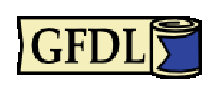
\includegraphics[width=1cm]{gfdl-logo-small.eps}
        \fi

Copyright (c) 2012  Laurent Claessens

Permission is granted to copy, distribute and/or modify this document under the terms of the \href{http://www.gnu.org/licenses/fdl-1.3.html}{GNU Free Documentation License}, Version 1.3 or any later version published by the Free Software Foundation; with no Invariant Sections, no Front-Cover Texts, and no Back-Cover Texts. A copy of the license is included in the chapter entitled ``GNU Free Documentation~License''.

\vspace{0.5cm}

Vous avez le droit de copier, distribuer et modifier ce document pourvu que vous suiviez les règles de la \wikipedia{fr}{GFDL}{GNU Free Documentation License}. Vous trouverez les sources \LaTeX\ sur gitorious :\\
    \url{https://www.gitorious.org/smath/smath/trees/master}

\end{center}


\tableofcontents

\newpage

\part{Seconde}

Je vais un peu suivre \cite{oklaEg}.

\chapter{Statistiques descriptives}
% This is part of Un soupçon de mathématique sans être agressif pour autant
% Copyright (c) 2012
%   Laurent Claessens
% See the file fdl-1.3.txt for copying conditions.


%+++++++++++++++++++++++++++++++++++++++++++++++++++++++++++++++++++++++++++++++++++++++++++++++++++++++++++++++++++++++++++
\section{Activité : mois de naissance}
%+++++++++++++++++++++++++++++++++++++++++++++++++++++++++++++++++++++++++++++++++++++++++++++++++++++++++++++++++++++++++++

Prendre les mois de naissance des élèves, en séparant les groupes.
\begin{enumerate}
    \item
        Quel groupe a la proportion de naissance en mars la plus grande ?
    \item
        En tout quelle est la proportion des naissances en avril ?
    \item 
        Est-ce qu'on peut voir l'effet comme quoi les mois de \( 31\) jours son plus longs ? 
        \begin{enumerate}
            \item
                Quelle est la proportion d'élèves nés dans un mois de \( 31\) jours ?
            \item
                Il y a \( 7\) mois de $31$ jours contre \( 5\) de moins. Donc le résultat est biaisé.
            \item
                Calculer la \emph{fréquence} des naissances en naissances par mois.
        \end{enumerate}
\end{enumerate}

%+++++++++++++++++++++++++++++++++++++++++++++++++++++++++++++++++++++++++++++++++++++++++++++++++++++++++++++++++++++++++++
\section{Regardons des graphiques}
%+++++++++++++++++++++++++++++++++++++++++++++++++++++++++++++++++++++++++++++++++++++++++++++++++++++++++++++++++++++++++++

Les graphiques sont souvent tirés de wikipédia. Si vous voulez plus d'informations, lisez \url{http://www.manicore.com/}, ou bien regardez le cours \href{http://www.mines-paristech.fr/ingenieurcivil/SitesIC/Balado/Climat_som.html}{en ligne}, en particulier la deuxième heure du troisième cours donne les facteurs d'émissions dans le monde et en France.

%---------------------------------------------------------------------------------------------------------------------------
\subsection{Émissions par secteurs}
%---------------------------------------------------------------------------------------------------------------------------

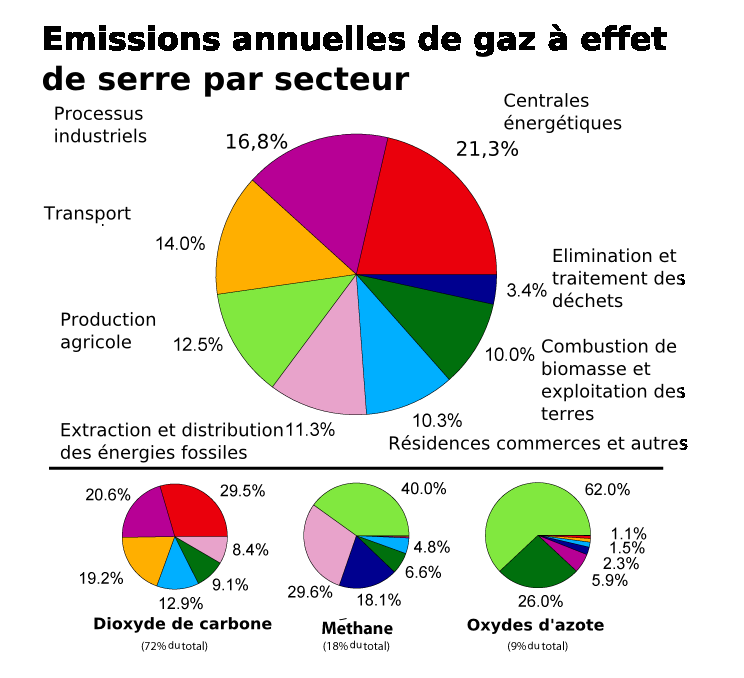
\includegraphics[width=17cm]{Emission_de_GES.png}
Graphique en provenance de l'article \wikipedia{fr}{Gaz_à_effet_de_serre}{gaz à effet de serre} de wikipédia.

\begin{enumerate}
    \item
        Quel est le secteur qui émets le plus ?
    \item
        Est-ce que l'agriculture émet beaucoup de dioxyde de carbone ?
    \item
        À partir des deux graphiques du bas, est-ce que vous êtes capables de retrouver le \( 12.5\%\) de l'agriculture donnés dans le graphique du haut ?
\end{enumerate}

%---------------------------------------------------------------------------------------------------------------------------
\subsection{Découvertes de pétrole}
%---------------------------------------------------------------------------------------------------------------------------

Regardons un instant le graphique suivant, provenant de l'article \wikipedia{fr}{Pic_pétrolier}{Pic pétrolier} de wikipédia.

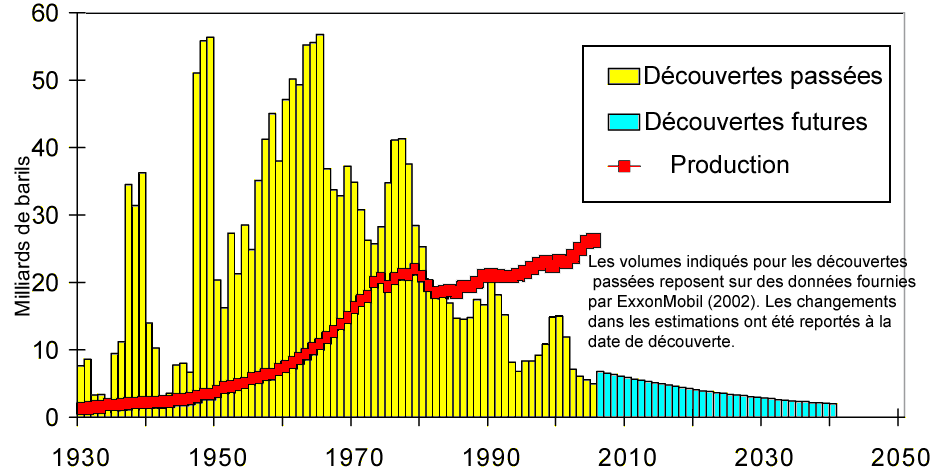
\includegraphics[width=17cm]{Decouvertes-petrole.png}

\begin{enumerate}
    \item
        Quelle est l'année où on a découvert le plus de pétrole ?
    \item
        Quelle est l'année où on a consommé le plus de pétrole ?
    \item
        En quelles années on a consommé autant qu'on a découvert ?
    \item
        Que pensez-vous de l'affirmation «ce qui reste comme réserve est la surface jaune au-dessus de la ligne rouge» ?
\end{enumerate}
Pour aller plus loin, remarquer la cassure assez nette de la croissance de la production vers 1975. Juste par curiosité, faites quelque recherches sur l'histoire de la croissance économique, de la dette publique et le chômage en France (et en Europe). Est-ce que les années 1970 ont été spéciales de ce point de vue ?

%---------------------------------------------------------------------------------------------------------------------------
\subsection{Températures}
%---------------------------------------------------------------------------------------------------------------------------

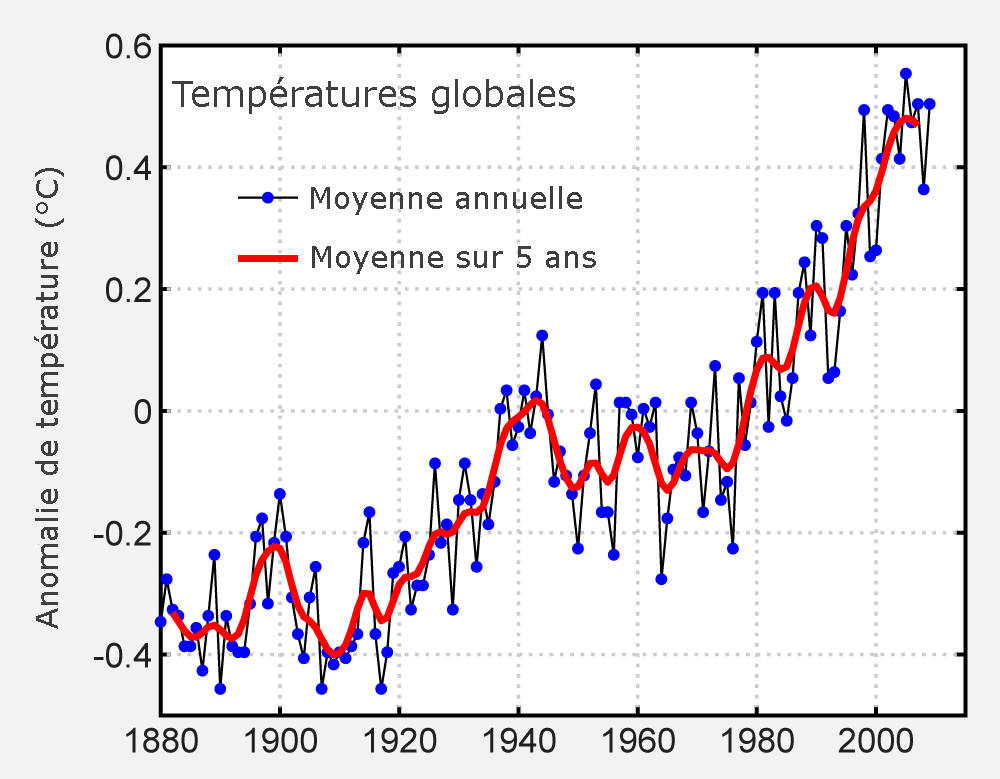
\includegraphics[width=17cm]{Instrumental_Temperature_Record_fr.png}
Graphique en provenance de l'article \wikipedia{fr}{Réchauffement_climatique}{réchauffement climatique} de wikipédia.

Le zéro de ce graphique est la moyenne 1961-1990.

\begin{enumerate}
    \item
        Quelle est la dernière année «normale» ?
    \item
        Quelle est l'année la plus chaude ?
    \item
        Quelle est l'année la plus froide ?
\end{enumerate}

%---------------------------------------------------------------------------------------------------------------------------
\subsection{Consommation de pétrole}
%---------------------------------------------------------------------------------------------------------------------------

Lire le tableau suivant :
\begin{center}
\begin{tabular}[h]{|c|c|c|c|c|c|c|c|c|}
année&
2001&
2002&
2003&
2004&
2005&
2006&
2007&
2008\\
consommation (Mb/j)&
76,8&
77,7&
79,1&
81,8&
83,1&
83,8&
84,9&
84,5
\end{tabular}
\end{center}

Calculer le pourcentage d'augmentation année par année. Que s'est-il passé en 2008 ?

%---------------------------------------------------------------------------------------------------------------------------
\subsection{À faire fonctionner}
%---------------------------------------------------------------------------------------------------------------------------

Les graphiques montrent
\begin{enumerate}
    \item

        À la figure \ref{LabelFigautomaticDSpcb}, \( y=\) proportion des étudiants ayant obtenu plus que \( x\)
    \item
        À la figure \ref{LabelFigautomaticDSpbt}, \( y=\) moyenne des étudiants ayant obtenu plus que \( x\). Par construction, le tout premier point de ce graphique est la moyenne de tout le groupe.
    \item
        À la figure \ref{LabelFigautomaticDSavb}, \( y=\) proportion des étudiants ayant obtenu dans \( \mathopen[ x-0.5 , x+0.5 \mathclose]\).
\end{enumerate}

\newcommand{\CaptionFigautomaticDSpcb}{Moyenne des étudiants ayant obtenus plus que \( x\)}
\input{Fig_automaticDSpcb.pstricks}

\newcommand{\CaptionFigautomaticDSpbt}{Proportion des étudiants ayant obtenus plus que \( x\)}
\input{Fig_automaticDSpbt.pstricks}

\newcommand{\CaptionFigautomaticDSavb}{proportion des étudiants ayant obtenu dans \( x\pm 0.5\)}
\input{Fig_automaticDSavb.pstricks}

%+++++++++++++++++++++++++++++++++++++++++++++++++++++++++++++++++++++++++++++++++++++++++++++++++++++++++++++++++++++++++++
\section{Théorie}
%+++++++++++++++++++++++++++++++++++++++++++++++++++++++++++++++++++++++++++++++++++++++++++++++++++++++++++++++++++++++++++

\begin{definition}
    Une \defe{population}{population} est un ensemble fini. Une \defe{série statistique}{série statistique} sur une population est une fonction qui à chaque élément (individu) de la population fait correspondre une valeur.

    L'\defe{effectif}{effectif} d'une valeur est le nombre d'individus correspondant à la valeur.

    La \defe{fréquence}{fréquence} d'une valeur est le rapport
    \begin{equation}
        f=\frac{ \text{effectif de la valeur} }{ \text{effectif total} }
    \end{equation}
    où par «effectif total» nous entendons la taille de la population totale.
\end{definition}

La \defe{moyenne}{moyenne} d'une suite de nombres \( x_1,\ldots, x_n\) est
\begin{equation}
    \bar x=\frac{1}{ n }\sum_{i=1}^nx_i=\frac{ \text{somme des \( x_i\)} }{\text{nombre de données}}.
\end{equation}

\begin{example}
    Soit la suite de nombres
    \begin{equation}
        1,7,0,3,9,0,1,3,1,0,2,5,6,9,1,1,3,2,4.
    \end{equation}
    Il y a \( 19\) nombres. La moyenne est donnée par la fraction
    \begin{equation}
        \bar x=\frac{ 1+7+0+3+9+\ldots+3+2+4 }{ 19 }=\frac{ 58 }{ 19 }.
    \end{equation}

Python permet d'obtenir assez facilement une approximation numérique :
    \begin{verbatim}
>>> import numpy
>>> nombres=[1,7,0,3,9,0,1,3,1,0,2,5,6,9,1,1,3,2,4]
>>> numpy.mean(nombres)          # 'mean' signifie 'moyenne' en anglais.
3.0526315789473686 
    \end{verbatim}
\end{example}

\begin{example}
    Voici un petit tableau de l'\href{http://www.insee.fr/fr/themes/tableau.asp?reg_id=0&ref_id=NATTEF13325}{INSEE}, parlant du chiffre d'affaire des éditeurs vidéos en million d'euros.

    \begin{center}
    \begin{tabular}{|c|c|c|c|c|c|}
        \hline
        &Vidéo à la demande &   \multicolumn{3}{| c |}{Vente}&Total\\
        \hline
        &                   &   total&dont DVD&dont Blu-ray&\\
        \hline
        2004&nd&1958.8&1844.6&&nd\\
        2005&nd&1784.2&1757.3&&nd\\
        2006&nd&1659.2&1654.7&&nd\\
        2007&28.9&1494.1&1479.9&14.3&1523.0\\
        2008&53.2&1382.4&1331.0&51.5&1435.6\\
        2009&97.0&1384.4&1277.1&107.3&1481.4\\
        2010&152.0&1385.4&1211.7&173.7&1537.4\\
        2011&219.5&1257.5&1048.4&209.1&1477\\
        \hline
    \end{tabular}
    \end{center}
    Dessiner un diagramme en camembert pour les années 2007 et 2011.
\end{example}

\chapter{Repères, distances, milieux}
% This is part of Un soupçon de mathématique sans être agressif pour autant
% Copyright (c) 2012
%   Laurent Claessens
% See the file fdl-1.3.txt for copying conditions.


%+++++++++++++++++++++++++++++++++++++++++++++++++++++++++++++++++++++++++++++++++++++++++++++++++++++++++++++++++++++++++++
\section{Repères}
%+++++++++++++++++++++++++++++++++++++++++++++++++++++++++++++++++++++++++++++++++++++++++++++++++++++++++++++++++++++++++++

%---------------------------------------------------------------------------------------------------------------------------
\subsection{Activité}
%---------------------------------------------------------------------------------------------------------------------------

Si nous plaçons un point sur le tableau, comment faire pour mettre un point au même endroit sur le tableau de la classe d'à côté ?

%---------------------------------------------------------------------------------------------------------------------------
\subsection{Repère}
%---------------------------------------------------------------------------------------------------------------------------

\begin{definition}
    Un \defe{repère orthonormé}{repère!orthonormé} du plan est la donné de trois points \( O\), \( I\), \( J\) non alignés formant un triangle rectangle isocèle en  \( O\).
\end{definition}

La façon dont nous associons à chaque point \( M\) du plan ses coordonnées dans le repère \( O\), \( I\), \( J\) est donnée à la figure \ref{LabelFigReperexjVyii}.
\newcommand{\CaptionFigReperexjVyii}{Lire les coordonnées du point \( M\) dans le repère \( OIJ\).}
\input{Fig_ReperexjVyii.pstricks}

%+++++++++++++++++++++++++++++++++++++++++++++++++++++++++++++++++++++++++++++++++++++++++++++++++++++++++++++++++++++++++++
\section{Milieu d'un segment}
%+++++++++++++++++++++++++++++++++++++++++++++++++++++++++++++++++++++++++++++++++++++++++++++++++++++++++++++++++++++++++++

\begin{example}
    Le tableau suivant recense différentes situations de points \( A\) et \( B\) dans le plan. Pour chaque cas, dessiner les points et trouver le milieu.

    \begin{center}
        \begin{tabular}[h]{|c||c|c|c|c|c|c|}
            \hline
            \( A\)&\( (3;0)\)&\( (2,7)\)&\( (1;1)\)&\( (0,0)\)&\( (-1,3)\)&\( (7;-8)\)\\
            \hline
            \( B\)&\( (7,0)\)&\( (2,5)\)&\( (3,3)\)&\( (3,4)\)&\( (1,-5)\)&\( (-6,1)\)\\
            \hline\hline
            milieu&&&&&\\
            \hline
        \end{tabular}
    \end{center}
\end{example}

\begin{Aretenir}
    Soient les points \( A\) et \( B\) de coordonnées \( A=(x_A,y_A)\) et \( B=(x_B,y_B)\) dans un repère. Alors le milieu du segment \( [AB]\) est le point de coordonnées
    \begin{equation}
        \begin{aligned}[]
            x_M&=\frac{ x_A+x_B }{ 2 },&y_M&=\frac{ y_A+y_B }{2}.
        \end{aligned}
    \end{equation}
\end{Aretenir}

%+++++++++++++++++++++++++++++++++++++++++++++++++++++++++++++++++++++++++++++++++++++++++++++++++++++++++++++++++++++++++++
\section{Distance entre deux points}
%+++++++++++++++++++++++++++++++++++++++++++++++++++++++++++++++++++++++++++++++++++++++++++++++++++++++++++++++++++++++++++

Lorsque \( A\) et \( B\) sont deux points du plan, nous notons \( \| AB \|\)\nomenclature{\( \| AB \|\)}{la longueur du segment \( [AB]\)} la longueur du segment \( [AB]\).
    \begin{Aretenir}
\begin{multicols}{2}
        Soient les points \( A\) et \( B\) de coordonnées \( A=(A_x,A_y)\) et \( B=(B_x,B_y)\) dans un repère orthonormé. La distance entre \( A\) et \( B\) (c'est à dire la longueur du segment \( [AB]\)) est donnée par la formule
        \begin{equation}
            \| AB \|=\sqrt{(A_x-B_x)^2+(A_y-B_y)^2}.
        \end{equation}
    
\columnbreak

\phantom{a} % Je ne suis pas très fier de ce moyen de faire arriver le dessin en bas de la colonne.

\vfill

%The result is on figure \ref{LabelFigPythagoreeBqLDU}.
%\newcommand{\CaptionFigPythagoreeBqLDU}{<+Type your caption here+>}
\input{Fig_PythagoreeBqLDU.pstricks}

\end{multicols}
    \end{Aretenir}



\begin{proof}
    Nous allons utiliser le théorème de Pythagore. Pour cela nous construisons le triangle rectangle construit sur les points \( A\) et \( B\) comme indiqué sur le dessin. Le point \( C\) est le point de même abscisse que \( B\) et de même ordonnée que \( A\), c'est à dire que \( C\) est le point
    \begin{equation}
        C=(B_x,A_y).
    \end{equation}
    La droite \( AC\) est parallèle à l'axe des abscisses et la droite \( BC\) est parallèle à l'axe des ordonnées; elles sont donc perpendiculaires et le triangle \( ABC\) est un triangle rectangle en \( C\). Le théorème de Pythagore s'applique :
    \begin{equation}    \label{EqjLjEKr}
       AB =\sqrt{ AC^2+BC^2}.
    \end{equation}
    Il reste à déterminer les longueurs \( \| AC \|\) et \( \| BC \|\). Le segment \( [AC]\) est horizontal et s'étend de l'abscisse \( A_x\) à l'abscisse \( B_x\), donc il est de longueur soit \( A_x-B_x\) soit \( B_x-A_x\), mais dans les deux cas nous avons
    \begin{equation}
        \| AC \|^2=(B_x-A_x)^2.
    \end{equation}
    De la même façon nous avons 
    \begin{equation}
        \| BC \|^2=(B_y-A_y)^2.
    \end{equation}
    En remplaçant dans \eqref{EqjLjEKr}, nous obtenons le résultat annoncé.
\end{proof}

%+++++++++++++++++++++++++++++++++++++++++++++++++++++++++++++++++++++++++++++++++++++++++++++++++++++++++++++++++++++++++++
\section{Exercices de géométrie repérée}
%+++++++++++++++++++++++++++++++++++++++++++++++++++++++++++++++++++++++++++++++++++++++++++++++++++++++++++++++++++++++++++

%---------------------------------------------------------------------------------------------------------------------------
\subsection{Géométrie brute}
%---------------------------------------------------------------------------------------------------------------------------

\Exo{Seconde-0045}
\Exo{smath-0010}

%---------------------------------------------------------------------------------------------------------------------------
\subsection{Placer et lire des coordonnées dans un repère}
%---------------------------------------------------------------------------------------------------------------------------

\Exo{Seconde-0001}
\Exo{Seconde-0002}
\Exo{Seconde-0007}
\Exo{Seconde-0062}

%---------------------------------------------------------------------------------------------------------------------------
\subsection{Milieu de segments}
%---------------------------------------------------------------------------------------------------------------------------

\Exo{Seconde-0056}
\Exo{Seconde-0012}
\Exo{Seconde-0055}
\Exo{Seconde-0011}

%---------------------------------------------------------------------------------------------------------------------------
\subsection{Longueur de segments}
%---------------------------------------------------------------------------------------------------------------------------

\Exo{Seconde-0008}
\Exo{Seconde-0003}
\Exo{Seconde-0004}
\Exo{Seconde-0005}
\Exo{Seconde-0006}
\Exo{Seconde-0009}
\Exo{Seconde-0010}
\Exo{Seconde-0013}
\Exo{Seconde-0021}
\Exo{Seconde-0019}
\Exo{Seconde-0020}

%---------------------------------------------------------------------------------------------------------------------------
\subsection{Problèmes}
%---------------------------------------------------------------------------------------------------------------------------

\Exo{Seconde-0077}
\Exo{Seconde-0078}
\Exo{Seconde-0079}
\Exo{Seconde-0080}
\Exo{Seconde-0081}
\Exo{Seconde-0082}
\Exo{Seconde-0083}
\Exo{Seconde-0084}
\Exo{Seconde-0085}
\Exo{Seconde-0098}
\Exo{Seconde-0099}
\Exo{Seconde-0100}


\part{Première STMG}
% This is part of Un soupçon de mathématique sans être agressif pour autant
% Copyright (c) 2012
%   Laurent Claessens
% See the file fdl-1.3.txt for copying conditions.

\chapter{Proportions, pourcentages}

%+++++++++++++++++++++++++++++++++++++++++++++++++++++++++++++++++++++++++++++++++++++++++++++++++++++++++++++++++++++++++++
\section{Théorie}
%+++++++++++++++++++++++++++++++++++++++++++++++++++++++++++++++++++++++++++++++++++++++++++++++++++++++++++++++++++++++++++

Nous disons qu'un gaz est en concentration de une \defe{partie par million}{partie par million} si un million de grammes d'air contient un gramme du gaz. Voici quelque chiffre concernant l'évolution de la concentration de \( CO_2\) dans l'atmosphère; les chiffres sont en \( \unit{}{ppm}\) :
\begin{center}
\begin{tabular}{|c|c|c|}
    \hline
    1750    &   2005    &   1012\\
    \hline
    280&380&395\\
    \hline
\end{tabular}
\end{center}
Pour information, cette concentration n'a pas dépassé les \unit{300}{ppm} depuis au moins \( 600.000\) ans.

\begin{enumerate}
    \item
        De combien de pourcent la concentration de \( CO_2\) a augmenté entre 1750 et 2005 ?
    \item
        Sur un kilo d'air, combien de grammes de \( CO_2\) ?
    \item 
        Quelle est la vitesse (en ppm par an) d'augmentation de la concentration entre 1750 et 2005 ? Même question entre 2005 et 2012.
\end{enumerate}

\begin{definition}
    Une \defe{population}{population} est un ensemble fini. Si \( E\) est une population, une \defe{sous-population}{sous-population} est un sous-ensemble \( A\subset E\). L'\defe{effectif}{effectif} d'une population est le nombre de ses éléments.

    La \defe{proportion}{proportion} de \( A\) dans \( E\) est le rapport
    \begin{equation}
        p_A=\frac{ n_A }{ n_E }
    \end{equation}
    où \( n_A\) et \( n_E\) sont les effectifs de \( A\) et \( E\).
\end{definition}
Note : une proportion est un nombre compris entre zéro et un.

\begin{example}
    Demander combien il y a de gauchers dans la classe. Quelle en est la proportion ?
\end{example}

\begin{example}
    Diviser la classe en \( 4\) groupes suivant que l'élève habite ou non à Dole et qu'il utilise ou non un cahier. Remplir le tableau suivant :

    \begin{center}
    \begin{tabular}{|l||c|c||c|}
        \hline\hline
        & habite à Dole&n'habite pas à Dole&total\\
        \hline
        utilise un cahier&&&\\
        \hline
        n'utilise pas de cahier&&&\\
        \hline\hline
        total&&&\\
        \hline
    \end{tabular}
    \end{center}

    Soit \( E\) la population totale : toute la classe; soit $A$ la population de ceux qui vivent à Dole; et \( B\) celle de ceux qui utilisent un cahier.
    \begin{enumerate}
        \item
            Trouver les effectifs des populations \( A\cup B\) et \( A\cap B\).
        \item
            Quelle est la proportion de \( A\) dans \( E\) ? Et celle du complémentaire \( \bar A\) ?
        \item
            Exprimer les proportions \( p_{A\cap B}\) et \( p_{A\cup B}\).
    \end{enumerate}
\end{example}

Nous avons l'égalité
\begin{equation}
    n_{A\cup B}=n_A+n_B-n_{A\cap B}
\end{equation}
parce que dans le compte \( n_A+n_B\), nous comptons deux fois les individus qui sont dans \( A\) et dans \( B\). En passant aux proportions (c'est à dire en divisant tout par \( n_E\)), nous avons la formule
\begin{equation}
    p_{A\cup B}=p_A+p_B-p_{A\cap B}.
\end{equation}

\begin{remark}
    Si les populations \( A\) et \( B\) sont disjointes, alors \( n_{A\cap B}=0\) et nous trouvons la formule
    \begin{equation}
        p_{A\cup B}=p_A+p_B.
    \end{equation}
\end{remark}


%+++++++++++++++++++++++++++++++++++++++++++++++++++++++++++++++++++++++++++++++++++++++++++++++++++++++++++++++++++++++++++
\section{Exercices}
%+++++++++++++++++++++++++++++++++++++++++++++++++++++++++++++++++++++++++++++++++++++++++++++++++++++++++++++++++++++++++++

\Exo{Seconde-0022}
\Exo{Seconde-0030}
\Exo{Premiere-0001}
\Exo{Premiere-0002}
\Exo{Premiere-0003}
\Exo{Premiere-0004}
\Exo{Premiere-0005}
\Exo{Premiere-0006}

\Exo{Premiere-0007}
\Exo{Premiere-0008}
\Exo{Premiere-0009}
\Exo{Premiere-0010}
\Exo{Premiere-0011}
\Exo{Premiere-0012}
\Exo{Seconde-0026}
\Exo{Seconde-0024}
\Exo{Premiere-0014}                                                                                                                                     
\Exo{Premiere-0015}                                               
\Exo{Premiere-0016}                                                                       
\Exo{Premiere-0017}                                                                                                                      
\Exo{Seconde-0034}

\Exo{Premiere-0023}                                                                                                                                    


\chapter{Second degré}

%+++++++++++++++++++++++++++++++++++++++++++++++++++++++++++++++++++++++++++++++++++++++++++++++++++++++++++++++++++++++++++
\section{Définitions}
%+++++++++++++++++++++++++++++++++++++++++++++++++++++++++++++++++++++++++++++++++++++++++++++++++++++++++++++++++++++++++++

\begin{definition}
    Une fonction \defe{polynôme de degré $2$}{polynôme (de degré $2$)} est une fonction s'exprimant sous la forme 
    \begin{equation}
    f(x)=ax^2+bx+c
    \end{equation}
    où \( a\), \( b\) et \( c\) sont des nombres réels avec \( a\neq 0\). 
    
    La courbe représentative d'un polynôme de degré deux dans un plan orthonormé est une \defe{parabole}{parabole}.
\end{definition}

%---------------------------------------------------------------------------------------------------------------------------
\subsection{Symétries, tableau de variations}
%---------------------------------------------------------------------------------------------------------------------------

La parabole de la fonction \( f(x)=ax^2+bx+c\) (\( a\neq 0\)) est symétrique par rapport à la droite d'équation \( x=-\frac{ b }{ 2a }\), c'est à dire par rapport à la droite verticale en \( x=-b/2a\). Le \defe{sommet}{sommet (d'une parabole)} est le point d'abscisse 
\begin{equation}
x=-b/2a
\end{equation}
situé sur la parabole.

Deux paraboles avec leurs axes de symétries sont dessinées à la figure \ref{LabelFigParaboles}.
\newcommand{\CaptionFigParaboles}{Deux paraboles}
\input{Fig_Paraboles.pstricks}

Comment savoir si les branches de la paraboles \( ax^2+bx+c\) sont orientées vers le haut ou vers le bas ? La règle est simple : 
\begin{enumerate}
    \item
        si \( a>0\), alors elles sont tournées vers le haut;
    \item
        si \( a<0\), alors elles sont tournées vers le bas.
\end{enumerate}
Cette règle est facile à retenir en pensant par exemple à la parabole \( x^2+bx+c\) où \( b\) et \( c\) sont raisonnables. Si nous prenons \( x=1000\), alors \( x^2\) vaut un million alors que les deux autres termes ne valent que de l'ordre du mille. Il est alors clair que la branche part vers l'infini.

\vbox{  % Le problème est que ceci apparaît proche du bord inférieur de la page, du coup il saut de colonne avant mon \columnbreak et l'effet est merdé.
\begin{multicols}{2}
    
    Le tableau de variations pour une parabole \( f(x)=ax^2+bx+c\) avec \( a>0\) se présente ainsi :
\begin{equation*}
\begin{array}[h]{|c||ccccc|}
    \hline
    x&-\infty&&x_0=-b/2a&&\infty\\
    \hline
    &\infty&&&&\infty\\
    f(x)&&\searrow&&\nearrow&\\
    &&&f(x_0)&&\\
    \hline
\end{array}
\end{equation*}

  \columnbreak

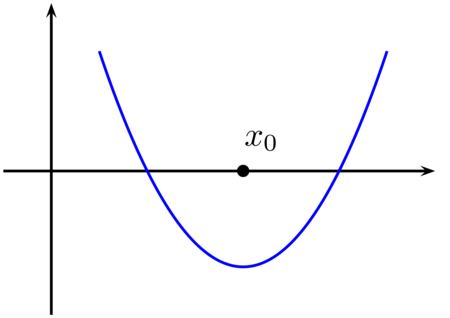
\includegraphics{Picture_FIGLabelFigParaboleHautMLbPQFPICTParaboleHautMLbPQF-for_eps.pdf}

\end{multicols}

}

\vbox{ 
\begin{multicols}{2}
    
    Le tableau de variations pour une parabole \( f(x)=ax^2+bx+c\) avec \( a<0\) se présente ainsi :
\begin{equation*}
\begin{array}[h]{|c||ccccc|}
    \hline
    x&-\infty&&x_0=-b/2a&&\infty\\
    \hline
    &&&f(x_0)&&\\
    f(x)&&\nearrow&&\searrow&\\
    &-\infty&&&&-\infty\\
    \hline
\end{array}
\end{equation*}


  \columnbreak

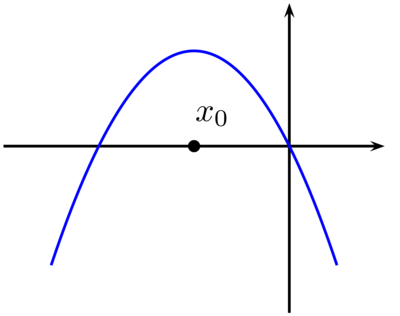
\includegraphics{Picture_FIGLabelFigParaboleBasfKtFCNPICTParaboleBasfKtFCN-for_eps.pdf}
\end{multicols}

}

%+++++++++++++++++++++++++++++++++++++++++++++++++++++++++++++++++++++++++++++++++++++++++++++++++++++++++++++++++++++++++++
\section{Tracer une parabole dont l'équation est connue}
%+++++++++++++++++++++++++++++++++++++++++++++++++++++++++++++++++++++++++++++++++++++++++++++++++++++++++++++++++++++++++++

Maintenant que les symétrie de la paraboles sont sont connues, il devient relativement facile d'en dessiner. Il est important d'être capable de tracer à main levée une courbe approximative passant par quelque points connus. SANS CALCULATRICE\footnote{Si vous me permettez une analogie, utiliser une calculatrice pour faire des études de fonctions, c'est comme utiliser un anti douleur pour améliorer ses performances sportives.}.

La méthode pour tracer la courbe représentative de \( f(x)=ax^2+bx+c\) se décompose en les pas suivants.
\begin{enumerate}
    \item
        D'abord il faut trouver le sommet de la parabole en utilisant la formule 
        \begin{equation}
            x_0=-\frac{ b }{ 2a }.
        \end{equation}
        Le somme est alors le point \( S=\big( x_0,f(x_0) \big)\).
    \item
        Tracer la droite verticale passant par le sommet; ce sera l'axe de symétrie.
    \item
        Dresser le tableau de variations de \( f\) en regardant le signe de \( a\). Si \( a\) est positif, le sommet sera le creux de la courbe; si \( a\) est négatif, alors le sommet sera un pic du graphique.
    \item
        Calculer quelque valeurs autour du sommet, par exemple \( x=0\), \( x=\pm1\).
    \item
        Tracer une belle courbe passant par les points calculés, ayant le bon axe de symétrie et le bon sommet.
\end{enumerate}

\begin{example}
    Traçons la courbe représentative de \( f(x)=x^2\). Ses paramètres sont \( a=1\), \( b=0\), \( c=0\); son axe de symétrie est donc \( x=0\), c'est à dire l'axe des ordonnées. Son sommet est le point \( S=(0,0)\) et le graphe passe par les points \( (-2,4)\), \( (-1,1)\), \( (0,0)\), \( (2,4)\). En repérant ces points sur la feuille, le tracé est aisé.

    Attention : c'est une courbe qui monte assez fort. Elle est tracée sur la figure \ref{LabelFigbDdpfh}.
\newcommand{\CaptionFigbDdpfh}{La courbe \( x\mapsto x^2\).}
\input{Fig_bDdpfh.pstricks}

\end{example}

\begin{example}
    Soit à tracer la courbe de \( f(x)=x^2-4x+3\).
    \begin{enumerate}
        \item
            Nous identifions \( a=1\), \( b=-4\), \( c=3\). 
        \item
            L'abscisse du sommet est \( x_0=-b/2a=\frac{ 4 }{2}=2\). Étant donné que \( f(2)=4-8+3=-1\), le sommet est en \( S=(2,-1)\).
        \item
            Calculons quelque points :
            \begin{itemize}
                \item \( f(1)=0\),
                \item
                    \( f(3)=0\),
                \item
                    \( f(0)=3\),
                \item
                    \( f(4)=3\).
            \end{itemize}
            Il est important de résister à la tentation de faire cette étape à la calculatrice tant que vous n'êtes pas complètement à l'aise.
        \item
            Placer les points \( (2,-1)\), \( (1,0)\), \( (3,0)\), \( (0,3)\) et \( (4,3)\) dans un plan.
        \item
            Tracer.
    \end{enumerate}
    Le résultat est tracé sur la figure \ref{LabelFigParabolevQzhjq}.
\newcommand{\CaptionFigParabolevQzhjq}{La courbe de la parabole \( x^2-4x+3\).}
\input{Fig_ParabolevQzhjq.pstricks}
\end{example}

\begin{example}
    Traçons la courbe de \( -x^2+4\). Une bonne chose à faire est de remarquer que cela est un produit remarquable :
    \begin{equation}
        f(x)=-(x+2)(x-2).
    \end{equation}
    Ceci va un peu nous simplifier la tâche parce que nous savons immédiatement les racines\footnote{Notons que nous n'avons pas encore montré comment trouver en général les racines d'un polynôme du second degré.} : \( \pm2\).
    %TODO : ajouter un lien vers là où ce sera fait

    Le sommet est en \( x_0=0\) et donc le sommet est \( S=(0,4)\). Nous pouvons encore calculer les points \( f(1)=3\) et \( f(3)=-5\). Avec cela nous pouvons tracer.

Le résultat est à la figure \ref{LabelFigParaboleiLbviP}.
\newcommand{\CaptionFigParaboleiLbviP}{La courbe de \( -x^2+4=-(x+2)(x-2)\).}
\input{Fig_ParaboleiLbviP.pstricks}

\end{example}

% TODO : À mettre quelque part : retenir que «parabole», «trinôme» et «polynôme du second degré», ce sont trois expressions essentiellement équivalentes.

%+++++++++++++++++++++++++++++++++++++++++++++++++++++++++++++++++++++++++++++++++++++++++++++++++++++++++++++++++++++++++++
\section{Donner l'équation d'une parabole dont deux racines sont connues}
%+++++++++++++++++++++++++++++++++++++++++++++++++++++++++++++++++++++++++++++++++++++++++++++++++++++++++++++++++++++++++++

\begin{example}
    Trouver une parabole qui s'annule en \( x=3\) et \( x=8\). Cela est très simple : il suffit d'écrire
    \begin{equation}
        f(x)=(x-3)(x-8).
    \end{equation}
    Le fait que cela s'annule en \( x=3\) et \( x=5\) est immédiat. En développant nous pouvons également l'écrire
    \begin{equation}
        f(x)=(x-3)(x-8)=x^2-8x-3x+24=x^2-11x+24.
    \end{equation}
    Le sommet de cette parabole est \( 11/2=5.5\). Remarquons encore que \( 5.5\) est juste au milieu de \( 3\) et \( 8\).
\end{example}

\begin{Aretenir}
    Les polynômes du second degré s'annulant en \( x=x_1\) et en \( x=x_2\) s'écrivent 
    \begin{equation}
        f(x)=m(x-x_1)(x-x_2)
    \end{equation}
    où \( m\) est n'importe quel réel.
\end{Aretenir}

Attention aux signes. Un polynôme qui s'annule en \( x=-1\) et \( x=-5\) s'écrit \( m(x+1)(x+5)\).

\begin{example}
    Un polynôme du second degré s'annulant en \( x=1\), en \( x=-2\) et dont le sommet est à la hauteur \( 5\). D'abord nous écrivons la forme générale du polynôme s'annulant en \( x=1\) et \( x=-2\) :
    \begin{equation}
        f(x)=m(x-1)(x+2).
    \end{equation}
    Nous développons : \( f(x)=m\big( x^2+x-2 \big)\). Le sommet de cette parabole est en \( x_S=-1/2\); notez que cela ne dépend pas de \( m\). Le sommet de la parabole est donc à la hauteur
    \begin{subequations}
        \begin{align}
            f(x_S)&=f\left( -\frac{ 1 }{2} \right)\\
            &=m\Big( \left( -\frac{ 1 }{2} \right)^2+\frac{ 1 }{2}-2 \Big)\\
            &=m\Big( \frac{1}{ 4 }+\frac{1}{ 2 }-2 \Big)\\
            &=-\frac{ 5m }{ 4 }.
        \end{align}
    \end{subequations}
    Nous devons fixer \( m\) pour que cette hauteur soit \( 5\), c'est à dire résoudre
    \begin{equation}
        -\frac{ 5m }{ 4 }=5,
    \end{equation}
    la solution est \( m=-4\). En définitive la fonction recherchée est
    \begin{equation}
        f(x)=-4x^2+4x-8.
    \end{equation}
\end{example}

%+++++++++++++++++++++++++++++++++++++++++++++++++++++++++++++++++++++++++++++++++++++++++++++++++++++++++++++++++++++++++++
\section{Équation du second degré}
%+++++++++++++++++++++++++++++++++++++++++++++++++++++++++++++++++++++++++++++++++++++++++++++++++++++++++++++++++++++++++++

Le gros morceau de ce chapitre est de déterminer les racines des polynômes\footnote{C'est à dire les \( x\) pour lesquels \( f(x)=0\)} du second degré. Les formules sont les suivantes.

\begin{Aretenir}
    Soit \( f(x)=ax^2+bx+c\) avec \( a\neq 0\). Les racines de \( f\) sont données par
    \begin{equation}    \label{EqmfNsjE}
        \begin{aligned}[]
            x_1&=\frac{ -b+\sqrt{b^2-4ac} }{ 2a }&\text{et}&&x_2&=\frac{ -b-\sqrt{b^2-4ac} }{ 2a }.
        \end{aligned}
    \end{equation}
\end{Aretenir}
Ces formules nécessitent de nombreux commentaires. Nous commençons par noter
\begin{equation}
    \Delta=b^2-4ac
\end{equation}
et appeler ce nombre le \defe{discriminant}{discriminant} de \( f\). Le discriminant va jouer un grand rôle dans l'étude des polynômes du second degré. Les deux racine de \( f\) s'écrivent 
\begin{equation}
    \frac{ -b\pm\sqrt{\Delta} }{ 2a }.
\end{equation}

Vérifions que le nombre \( x_1\) est bien une racine de \( ax^2+bx+c\). Pour cela nous devons calculer \( ax_1^2+bx_1+c\) en y substituant la valeur de \( x_1\). Le calcul est un peu long :
\begin{subequations}
    \begin{align}
        ax_1^2+bx_1+c&=a\left( \frac{ -b+\sqrt{\Delta} }{ 2a } \right)^2+b\left( \frac{ -b+\sqrt{\Delta} }{ 2a } \right)+c\\
        &=\frac{ a }{ 4a^2 }\big( b^2-2b\sqrt{\Delta}+b^2-4ac \big)+\frac{ b }{ 2a }\big( -b+\sqrt{\Delta} \big)+c&\text{développement du carré}\\
        &=\frac{1}{ 4a }\big( 2b^2-2b\sqrt{\Delta}-4ac \big)-\frac{ b^2 }{ 2a }+\frac{ b\sqrt{\Delta} }{ 2a }+c\\
        &=\frac{ b^2 }{ 2a }-\frac{ b\sqrt{\Delta} }{ 2a }-c-\frac{ b^2 }{ 2a }+\frac{ b\sqrt{\Delta} }{ 2a }+c\\
        =&0
    \end{align}
\end{subequations}

%---------------------------------------------------------------------------------------------------------------------------
\subsection{Exemple quand tout va bien}
%---------------------------------------------------------------------------------------------------------------------------

\begin{example} \label{ExgMRBJJ}
    Trouver les racines de \( f(x)=x^2+2x-3\). Nous calculons le discriminant
    \begin{equation}
        \Delta=b^2-4\times a\times c=4-4\times 1\times (-3)=16.
    \end{equation}
    Donc \( \sqrt{\Delta}=4\). Les solutions sont donc
    \begin{equation}
        \frac{ -2+4 }{ 2 }=1
    \end{equation}
    et
    \begin{equation}
        \frac{ -2-4 }{ 2 }=-3.
    \end{equation}
    Le polynôme \( x^2+2x-3\) s'annule donc pour \( x=1\) et \( x=-3\).

    Conseil : le vérifier en remplaçant \( x\) par \( 1\) puis par \( -3\) dans la fonction donnée !!

    Le graphe de cette fonction est donné à la figure \ref{LabelFigParabolezBeHFl}. Notez le sommet en \( x_0=-b/2a=-1\).
    \newcommand{\CaptionFigParabolezBeHFl}{Graphe de la fonction \( f(x)=x^2+2x-3\) pour l'exemple \ref{ExgMRBJJ}.}
\input{Fig_ParabolezBeHFl.pstricks}
\end{example}

%---------------------------------------------------------------------------------------------------------------------------
\subsection{Exemple quand tout va mal}
%---------------------------------------------------------------------------------------------------------------------------

\newcommand{\CaptionFigParabolezmMGdN}{La parabole \( (x+1)^2+1\)}
\input{Fig_ParabolezmMGdN.pstricks}
Il existe des paraboles n'ayant pas de racines. Par exemple la fonction
\begin{equation}
    f(x)=(x+1)^2+1
\end{equation}
dont un dessin est donné à figure \ref{LabelFigParabolezmMGdN} ne s'annule pas parce que c'est un carré (toujours positif ou nul) plus \( 3\). Les formules \eqref{EqmfNsjE} sont-elles en défaut ? Voyons cela. D'abord nous développons le carré pour mettre \( f\) sous forme «usuelle» \( ax^2+bx+c\) :
\begin{equation}
    f(x)=(x+1)^2+1=x^2+2x+1+1=x^2+2x+2.
\end{equation}
Le discriminant est
\begin{equation}
    \Delta=4-4\times 1\times 2=4-8=-4.
\end{equation}
Il n'est donc pas possible de calculer \( \sqrt{\Delta}\) vu qu'il n'est pas possible de calculer des racines de nombres négatifs.


%+++++++++++++++++++++++++++++++++++++++++++++++++++++++++++++++++++++++++++++++++++++++++++++++++++++++++++++++++++++++++++
\section{Factorisation du trinôme du second degré}
%+++++++++++++++++++++++++++++++++++++++++++++++++++++++++++++++++++++++++++++++++++++++++++++++++++++++++++++++++++++++++++

<++>


%+++++++++++++++++++++++++++++++++++++++++++++++++++++++++++++++++++++++++++++++++++++++++++++++++++++++++++++++++++++++++++
\section{Exercices sur le second degré}
%+++++++++++++++++++++++++++++++++++++++++++++++++++++++++++++++++++++++++++++++++++++++++++++++++++++++++++++++++++++++++++

\Exo{Premiere-0030}
\Exo{Premiere-0031}
\Exo{Premiere-0032}

\Exo{Premiere-0041}

\Exo{Premiere-0042}
\Exo{Premiere-0024}                                                                                                                                  
\Exo{Premiere-0040}


% Résolution
\Exo{Premiere-0026}                                                                                               
\Exo{Premiere-0043}
\Exo{Premiere-0044}

%---------------------------------------------------------------------------------------------------------------------------
\subsection{Plus compliqués}
%---------------------------------------------------------------------------------------------------------------------------

\Exo{Premiere-0025}                                                                                                                                   
\Exo{Premiere-0028}
\Exo{Premiere-0029}


\part{Autres}
% This is part of Un soupçon de mathématique sans être agressif pour autant
% Copyright (c) 2013
%   Laurent Claessens
% See the file fdl-1.3.txt for copying conditions.



%+++++++++++++++++++++++++++++++++++++++++++++++++++++++++++++++++++++++++++++++++++++++++++++++++++++++++++++++++++++++++++ 
\section{Exercices pour TSTL}
%+++++++++++++++++++++++++++++++++++++++++++++++++++++++++++++++++++++++++++++++++++++++++++++++++++++++++++++++++++++++++++
% Les quatre premiers ont été donnés en colle.
\Exo{smath-0283}
\Exo{smath-0284}
\Exo{smath-0285}
\Exo{smath-0286}
\Exo{smath-0415}
\Exo{smath-0416}

%+++++++++++++++++++++++++++++++++++++++++++++++++++++++++++++++++++++++++++++++++++++++++++++++++++++++++++++++++++++++++++ 
\section{Sujets de dissertations}
%+++++++++++++++++++++++++++++++++++++++++++++++++++++++++++++++++++++++++++++++++++++++++++++++++++++++++++++++++++++++++++

\Exo{smath-0418}
\Exo{smath-0419}
\Exo{smath-0420}

\Exo{smath-0423}
\Exo{smath-0424}
\Exo{smath-0425}
\Exo{smath-0426}
\Exo{smath-0427}
\Exo{smath-0428}
\Exo{smath-0429}
\Exo{smath-0430}

%+++++++++++++++++++++++++++++++++++++++++++++++++++++++++++++++++++++++++++++++++++++++++++++++++++++++++++++++++++++++++++ 
\section{Suites arithmétiques}
%+++++++++++++++++++++++++++++++++++++++++++++++++++++++++++++++++++++++++++++++++++++++++++++++++++++++++++++++++++++++++++

Une suite arithmétique peut également être écrite sous forme «non récurrence». Soit la suite arithmétique
\begin{subequations}
    \begin{numcases}{}
        u_0=2\\
        u_{n+1}=u_n+3.
    \end{numcases}
\end{subequations}
Nous avons \( u_1=2+3\), \( u_2=2+3+3\), \( u_3=2+3+3+3\), etc. Donc \( u_n=2+3n\). Plus généralement pour une suite dont le terme initial est \( u_0\) et la raison vaut \( a\), nous avons
\begin{equation}
    u_n=u_0+na.
\end{equation}
Si par contre le terme initial est \( u_1\), alors nous avons
\begin{equation}
    u_n=u_1+(n-1)a.
\end{equation}
Ce qui est important à retenir est que la raison d'une suite arithmétique est le multiple de \( n\).


\corrChapitre{Corrigés systématiques}

\chapter{GNU Free Documentation License}

 \begin{center}

       Version 1.3, 3 November 2008


 Copyright \copyright{} 2000, 2001, 2002, 2007, 2008  Free Software Foundation, Inc.
 
 \bigskip

 \href{http://fsf.org/}{http://fsf.org/} 

 \bigskip
 
 Everyone is permitted to copy and distribute verbatim copies
 of this license document, but changing it is not allowed.
\end{center}

%---------------------------------------------------------------------------------------------------------------------------
\section*{Preamble}
%---------------------------------------------------------------------------------------------------------------------------

The purpose of this License is to make a manual, textbook, or other
functional and useful document ``free'' in the sense of freedom: to
assure everyone the effective freedom to copy and redistribute it,
with or without modifying it, either commercially or noncommercially.
Secondarily, this License preserves for the author and publisher a way
to get credit for their work, while not being considered responsible
for modifications made by others.

This License is a kind of ``copyleft'', which means that derivative
works of the document must themselves be free in the same sense.  It
complements the GNU General Public License, which is a copyleft
license designed for free software.

We have designed this License in order to use it for manuals for free
software, because free software needs free documentation: a free
program should come with manuals providing the same freedoms that the
software does.  But this License is not limited to software manuals;
it can be used for any textual work, regardless of subject matter or
whether it is published as a printed book.  We recommend this License
principally for works whose purpose is instruction or reference.

%---------------------------------------------------------------------------------------------------------------------------
\section*{APPLICABILITY AND DEFINITIONS}
%---------------------------------------------------------------------------------------------------------------------------

This License applies to any manual or other work, in any medium, that
contains a notice placed by the copyright holder saying it can be
distributed under the terms of this License.  Such a notice grants a
world-wide, royalty-free license, unlimited in duration, to use that
work under the conditions stated herein.  The ``\textbf{Document}'', below,
refers to any such manual or work.  Any member of the public is a
licensee, and is addressed as ``\textbf{you}''.  You accept the license if you
copy, modify or distribute the work in a way requiring permission
under copyright law.

A ``\textbf{Modified Version}'' of the Document means any work containing the
Document or a portion of it, either copied verbatim, or with
modifications and/or translated into another language.

A ``\textbf{Secondary Section}'' is a named appendix or a front-matter section of
the Document that deals exclusively with the relationship of the
publishers or authors of the Document to the Document's overall subject
(or to related matters) and contains nothing that could fall directly
within that overall subject.  (Thus, if the Document is in part a
textbook of mathematics, a Secondary Section may not explain any
mathematics.)  The relationship could be a matter of historical
connection with the subject or with related matters, or of legal,
commercial, philosophical, ethical or political position regarding
them.

The ``\textbf{Invariant Sections}'' are certain Secondary Sections whose titles
are designated, as being those of Invariant Sections, in the notice
that says that the Document is released under this License.  If a
section does not fit the above definition of Secondary then it is not
allowed to be designated as Invariant.  The Document may contain zero
Invariant Sections.  If the Document does not identify any Invariant
Sections then there are none.

The ``\textbf{Cover Texts}'' are certain short passages of text that are listed,
as Front-Cover Texts or Back-Cover Texts, in the notice that says that
the Document is released under this License.  A Front-Cover Text may
be at most 5 words, and a Back-Cover Text may be at most 25 words.

A ``\textbf{Transparent}'' copy of the Document means a machine-readable copy,
represented in a format whose specification is available to the
general public, that is suitable for revising the document
straightforwardly with generic text editors or (for images composed of
pixels) generic paint programs or (for drawings) some widely available
drawing editor, and that is suitable for input to text formatters or
for automatic translation to a variety of formats suitable for input
to text formatters.  A copy made in an otherwise Transparent file
format whose markup, or absence of markup, has been arranged to thwart
or discourage subsequent modification by readers is not Transparent.
An image format is not Transparent if used for any substantial amount
of text.  A copy that is not ``Transparent'' is called ``\textbf{Opaque}''.

Examples of suitable formats for Transparent copies include plain
ASCII without markup, Texinfo input format, LaTeX input format, SGML
or XML using a publicly available DTD, and standard-conforming simple
HTML, PostScript or PDF designed for human modification.  Examples of
transparent image formats include PNG, XCF and JPG.  Opaque formats
include proprietary formats that can be read and edited only by
proprietary word processors, SGML or XML for which the DTD and/or
processing tools are not generally available, and the
machine-generated HTML, PostScript or PDF produced by some word
processors for output purposes only.

The ``\textbf{Title Page}'' means, for a printed book, the title page itself,
plus such following pages as are needed to hold, legibly, the material
this License requires to appear in the title page.  For works in
formats which do not have any title page as such, ``Title Page'' means
the text near the most prominent appearance of the work's title,
preceding the beginning of the body of the text.

The ``\textbf{publisher}'' means any person or entity that distributes
copies of the Document to the public.

A section ``\textbf{Entitled XYZ}'' means a named subunit of the Document whose
title either is precisely XYZ or contains XYZ in parentheses following
text that translates XYZ in another language.  (Here XYZ stands for a
specific section name mentioned below, such as ``\textbf{Acknowledgements}'',
``\textbf{Dedications}'', ``\textbf{Endorsements}'', or ``\textbf{History}''.)  
To ``\textbf{Preserve the Title}''
of such a section when you modify the Document means that it remains a
section ``Entitled XYZ'' according to this definition.

The Document may include Warranty Disclaimers next to the notice which
states that this License applies to the Document.  These Warranty
Disclaimers are considered to be included by reference in this
License, but only as regards disclaiming warranties: any other
implication that these Warranty Disclaimers may have is void and has
no effect on the meaning of this License.

%---------------------------------------------------------------------------------------------------------------------------
\section*{VERBATIM COPYING}
%---------------------------------------------------------------------------------------------------------------------------

You may copy and distribute the Document in any medium, either
commercially or noncommercially, provided that this License, the
copyright notices, and the license notice saying this License applies
to the Document are reproduced in all copies, and that you add no other
conditions whatsoever to those of this License.  You may not use
technical measures to obstruct or control the reading or further
copying of the copies you make or distribute.  However, you may accept
compensation in exchange for copies.  If you distribute a large enough
number of copies you must also follow the conditions in section~3.

You may also lend copies, under the same conditions stated above, and
you may publicly display copies.

%---------------------------------------------------------------------------------------------------------------------------
\section*{COPYING IN QUANTITY}
%---------------------------------------------------------------------------------------------------------------------------


If you publish printed copies (or copies in media that commonly have
printed covers) of the Document, numbering more than 100, and the
Document's license notice requires Cover Texts, you must enclose the
copies in covers that carry, clearly and legibly, all these Cover
Texts: Front-Cover Texts on the front cover, and Back-Cover Texts on
the back cover.  Both covers must also clearly and legibly identify
you as the publisher of these copies.  The front cover must present
the full title with all words of the title equally prominent and
visible.  You may add other material on the covers in addition.
Copying with changes limited to the covers, as long as they preserve
the title of the Document and satisfy these conditions, can be treated
as verbatim copying in other respects.

If the required texts for either cover are too voluminous to fit
legibly, you should put the first ones listed (as many as fit
reasonably) on the actual cover, and continue the rest onto adjacent
pages.

If you publish or distribute Opaque copies of the Document numbering
more than 100, you must either include a machine-readable Transparent
copy along with each Opaque copy, or state in or with each Opaque copy
a computer-network location from which the general network-using
public has access to download using public-standard network protocols
a complete Transparent copy of the Document, free of added material.
If you use the latter option, you must take reasonably prudent steps,
when you begin distribution of Opaque copies in quantity, to ensure
that this Transparent copy will remain thus accessible at the stated
location until at least one year after the last time you distribute an
Opaque copy (directly or through your agents or retailers) of that
edition to the public.

It is requested, but not required, that you contact the authors of the
Document well before redistributing any large number of copies, to give
them a chance to provide you with an updated version of the Document.

%---------------------------------------------------------------------------------------------------------------------------
\section*{MODIFICATIONS}
%---------------------------------------------------------------------------------------------------------------------------

You may copy and distribute a Modified Version of the Document under
the conditions of sections 2 and 3 above, provided that you release
the Modified Version under precisely this License, with the Modified
Version filling the role of the Document, thus licensing distribution
and modification of the Modified Version to whoever possesses a copy
of it.  In addition, you must do these things in the Modified Version:

\begin{itemize}
\item[A.] 
   Use in the Title Page (and on the covers, if any) a title distinct
   from that of the Document, and from those of previous versions
   (which should, if there were any, be listed in the History section
   of the Document).  You may use the same title as a previous version
   if the original publisher of that version gives permission.
   
\item[B.]
   List on the Title Page, as authors, one or more persons or entities
   responsible for authorship of the modifications in the Modified
   Version, together with at least five of the principal authors of the
   Document (all of its principal authors, if it has fewer than five),
   unless they release you from this requirement.
   
\item[C.]
   State on the Title page the name of the publisher of the
   Modified Version, as the publisher.
   
\item[D.]
   Preserve all the copyright notices of the Document.
   
\item[E.]
   Add an appropriate copyright notice for your modifications
   adjacent to the other copyright notices.
   
\item[F.]
   Include, immediately after the copyright notices, a license notice
   giving the public permission to use the Modified Version under the
   terms of this License, in the form shown in the Addendum below.
   
\item[G.]
   Preserve in that license notice the full lists of Invariant Sections
   and required Cover Texts given in the Document's license notice.
   
\item[H.]
   Include an unaltered copy of this License.
   
\item[I.]
   Preserve the section Entitled ``History'', Preserve its Title, and add
   to it an item stating at least the title, year, new authors, and
   publisher of the Modified Version as given on the Title Page.  If
   there is no section Entitled ``History'' in the Document, create one
   stating the title, year, authors, and publisher of the Document as
   given on its Title Page, then add an item describing the Modified
   Version as stated in the previous sentence.
   
\item[J.]
   Preserve the network location, if any, given in the Document for
   public access to a Transparent copy of the Document, and likewise
   the network locations given in the Document for previous versions
   it was based on.  These may be placed in the ``History'' section.
   You may omit a network location for a work that was published at
   least four years before the Document itself, or if the original
   publisher of the version it refers to gives permission.
   
\item[K.]
   For any section Entitled ``Acknowledgements'' or ``Dedications'',
   Preserve the Title of the section, and preserve in the section all
   the substance and tone of each of the contributor acknowledgements
   and/or dedications given therein.
   
\item[L.]
   Preserve all the Invariant Sections of the Document,
   unaltered in their text and in their titles.  Section numbers
   or the equivalent are not considered part of the section titles.
   
\item[M.]
   Delete any section Entitled ``Endorsements''.  Such a section
   may not be included in the Modified Version.
   
\item[N.]
   Do not retitle any existing section to be Entitled ``Endorsements''
   or to conflict in title with any Invariant Section.
   
\item[O.]
   Preserve any Warranty Disclaimers.
\end{itemize}

If the Modified Version includes new front-matter sections or
appendices that qualify as Secondary Sections and contain no material
copied from the Document, you may at your option designate some or all
of these sections as invariant.  To do this, add their titles to the
list of Invariant Sections in the Modified Version's license notice.
These titles must be distinct from any other section titles.

You may add a section Entitled ``Endorsements'', provided it contains
nothing but endorsements of your Modified Version by various
parties---for example, statements of peer review or that the text has
been approved by an organization as the authoritative definition of a
standard.

You may add a passage of up to five words as a Front-Cover Text, and a
passage of up to 25 words as a Back-Cover Text, to the end of the list
of Cover Texts in the Modified Version.  Only one passage of
Front-Cover Text and one of Back-Cover Text may be added by (or
through arrangements made by) any one entity.  If the Document already
includes a cover text for the same cover, previously added by you or
by arrangement made by the same entity you are acting on behalf of,
you may not add another; but you may replace the old one, on explicit
permission from the previous publisher that added the old one.

The author(s) and publisher(s) of the Document do not by this License
give permission to use their names for publicity for or to assert or
imply endorsement of any Modified Version.

%---------------------------------------------------------------------------------------------------------------------------
\section*{COMBINING DOCUMENTS}
%---------------------------------------------------------------------------------------------------------------------------

You may combine the Document with other documents released under this
License, under the terms defined in section~4 above for modified
versions, provided that you include in the combination all of the
Invariant Sections of all of the original documents, unmodified, and
list them all as Invariant Sections of your combined work in its
license notice, and that you preserve all their Warranty Disclaimers.

The combined work need only contain one copy of this License, and
multiple identical Invariant Sections may be replaced with a single
copy.  If there are multiple Invariant Sections with the same name but
different contents, make the title of each such section unique by
adding at the end of it, in parentheses, the name of the original
author or publisher of that section if known, or else a unique number.
Make the same adjustment to the section titles in the list of
Invariant Sections in the license notice of the combined work.

In the combination, you must combine any sections Entitled ``History''
in the various original documents, forming one section Entitled
``History''; likewise combine any sections Entitled ``Acknowledgements'',
and any sections Entitled ``Dedications''.  You must delete all sections
Entitled ``Endorsements''.

%---------------------------------------------------------------------------------------------------------------------------
\section*{COLLECTIONS OF DOCUMENTS}
%---------------------------------------------------------------------------------------------------------------------------

You may make a collection consisting of the Document and other documents
released under this License, and replace the individual copies of this
License in the various documents with a single copy that is included in
the collection, provided that you follow the rules of this License for
verbatim copying of each of the documents in all other respects.

You may extract a single document from such a collection, and distribute
it individually under this License, provided you insert a copy of this
License into the extracted document, and follow this License in all
other respects regarding verbatim copying of that document.

%---------------------------------------------------------------------------------------------------------------------------
\section*{AGGREGATION WITH INDEPENDENT WORKS}
%---------------------------------------------------------------------------------------------------------------------------

A compilation of the Document or its derivatives with other separate
and independent documents or works, in or on a volume of a storage or
distribution medium, is called an ``aggregate'' if the copyright
resulting from the compilation is not used to limit the legal rights
of the compilation's users beyond what the individual works permit.
When the Document is included in an aggregate, this License does not
apply to the other works in the aggregate which are not themselves
derivative works of the Document.

If the Cover Text requirement of section~3 is applicable to these
copies of the Document, then if the Document is less than one half of
the entire aggregate, the Document's Cover Texts may be placed on
covers that bracket the Document within the aggregate, or the
electronic equivalent of covers if the Document is in electronic form.
Otherwise they must appear on printed covers that bracket the whole
aggregate.

%---------------------------------------------------------------------------------------------------------------------------
\section*{TRANSLATION}
%---------------------------------------------------------------------------------------------------------------------------

Translation is considered a kind of modification, so you may
distribute translations of the Document under the terms of section~4.
Replacing Invariant Sections with translations requires special
permission from their copyright holders, but you may include
translations of some or all Invariant Sections in addition to the
original versions of these Invariant Sections.  You may include a
translation of this License, and all the license notices in the
Document, and any Warranty Disclaimers, provided that you also include
the original English version of this License and the original versions
of those notices and disclaimers.  In case of a disagreement between
the translation and the original version of this License or a notice
or disclaimer, the original version will prevail.

If a section in the Document is Entitled ``Acknowledgements'',
``Dedications'', or ``History'', the requirement (section~4) to Preserve
its Title (section~1) will typically require changing the actual
title.

%---------------------------------------------------------------------------------------------------------------------------
\section*{TERMINATION}
%---------------------------------------------------------------------------------------------------------------------------

You may not copy, modify, sublicense, or distribute the Document
except as expressly provided under this License.  Any attempt
otherwise to copy, modify, sublicense, or distribute it is void, and
will automatically terminate your rights under this License.

However, if you cease all violation of this License, then your license
from a particular copyright holder is reinstated (a) provisionally,
unless and until the copyright holder explicitly and finally
terminates your license, and (b) permanently, if the copyright holder
fails to notify you of the violation by some reasonable means prior to
60 days after the cessation.

Moreover, your license from a particular copyright holder is
reinstated permanently if the copyright holder notifies you of the
violation by some reasonable means, this is the first time you have
received notice of violation of this License (for any work) from that
copyright holder, and you cure the violation prior to 30 days after
your receipt of the notice.

Termination of your rights under this section does not terminate the
licenses of parties who have received copies or rights from you under
this License.  If your rights have been terminated and not permanently
reinstated, receipt of a copy of some or all of the same material does
not give you any rights to use it.


%---------------------------------------------------------------------------------------------------------------------------
\section*{FUTURE REVISIONS OF THIS LICENSE}
%---------------------------------------------------------------------------------------------------------------------------

The Free Software Foundation may publish new, revised versions
of the GNU Free Documentation License from time to time.  Such new
versions will be similar in spirit to the present version, but may
differ in detail to address new problems or concerns.  See
\href{http://www.gnu.org/copyleft/}{http://www.gnu.org/copyleft/} .

Each version of the License is given a distinguishing version number.
If the Document specifies that a particular numbered version of this
License ``or any later version'' applies to it, you have the option of
following the terms and conditions either of that specified version or
of any later version that has been published (not as a draft) by the
Free Software Foundation.  If the Document does not specify a version
number of this License, you may choose any version ever published (not
as a draft) by the Free Software Foundation.  If the Document
specifies that a proxy can decide which future versions of this
License can be used, that proxy's public statement of acceptance of a
version permanently authorizes you to choose that version for the
Document.

%---------------------------------------------------------------------------------------------------------------------------
\section*{RELICENSING}
%---------------------------------------------------------------------------------------------------------------------------


``Massive Multiauthor Collaboration Site'' (or ``MMC Site'') means any
World Wide Web server that publishes copyrightable works and also
provides prominent facilities for anybody to edit those works.  A
public wiki that anybody can edit is an example of such a server.  A
``Massive Multiauthor Collaboration'' (or ``MMC'') contained in the
site means any set of copyrightable works thus published on the MMC
site.

``CC-BY-SA'' means the Creative Commons Attribution-Share Alike 3.0
license published by Creative Commons Corporation, a not-for-profit
corporation with a principal place of business in San Francisco,
California, as well as future copyleft versions of that license
published by that same organization.

``Incorporate'' means to publish or republish a Document, in whole or
in part, as part of another Document.

An MMC is ``eligible for relicensing'' if it is licensed under this
License, and if all works that were first published under this License
somewhere other than this MMC, and subsequently incorporated in whole
or in part into the MMC, (1) had no cover texts or invariant sections,
and (2) were thus incorporated prior to November 1, 2008.

The operator of an MMC Site may republish an MMC contained in the site
under CC-BY-SA on the same site at any time before August 1, 2009,
provided the MMC is eligible for relicensing.

%---------------------------------------------------------------------------------------------------------------------------
\section*{ADDENDUM: How to use this License for your documents}
%---------------------------------------------------------------------------------------------------------------------------

To use this License in a document you have written, include a copy of
the License in the document and put the following copyright and
license notices just after the title page:

\bigskip
\begin{quote}
    Copyright \copyright{}  YEAR  YOUR NAME.
    Permission is granted to copy, distribute and/or modify this document
    under the terms of the GNU Free Documentation License, Version 1.3
    or any later version published by the Free Software Foundation;
    with no Invariant Sections, no Front-Cover Texts, and no Back-Cover Texts.
    A copy of the license is included in the section entitled ``GNU
    Free Documentation License''.
\end{quote}
\bigskip
    
If you have Invariant Sections, Front-Cover Texts and Back-Cover Texts,
replace the ``with \dots\ Texts.'' line with this:

\bigskip
\begin{quote}
    with the Invariant Sections being LIST THEIR TITLES, with the
    Front-Cover Texts being LIST, and with the Back-Cover Texts being LIST.
\end{quote}
\bigskip
    
If you have Invariant Sections without Cover Texts, or some other
combination of the three, merge those two alternatives to suit the
situation.

If your document contains nontrivial examples of program code, we
recommend releasing these examples in parallel under your choice of
free software license, such as the GNU General Public License,
to permit their use in free software.



\bibliographystyle{unsrt}           % unsrt fait que la biblio arrive dans l'ordre de citation au lieu de l'ordre alphabétique.
\bibliography{mazhe}

\addcontentsline{toc}{chapter}{Liste des notations}

\printnomenclature

\printindex

\end{document}

\Exo{Premiere-0017}                                                                                                                      
\Exo{Premiere-0018}                                                                                                                                
\Exo{Premiere-0019}                                                                                                                              
\Exo{Premiere-0020}                                                                                                                                    
\Exo{Premiere-0021}                                                                                                                                    
\Exo{Premiere-0022}                                                                                                                                
\Exo{Premiere-0023}                                                                                                                                    
\Exo{Premiere-0024}                                                                                                                                  
\Exo{Premiere-0025}                                                                                                                                   
\Exo{Premiere-0026}                                                                                               
\Exo{Premiere-0027}
\Exo{Premiere-0028}
\Exo{Premiere-0029}
\Exo{Premiere-0030}
\Exo{Premiere-0031}
\Exo{Premiere-0032}
\Exo{Premiere-0033}
\Exo{Premiere-0034}
\Exo{Premiere-0035}
\Exo{Premiere-0036}
\Exo{Premiere-0037}
\Exo{Premiere-0038}
\Exo{Premiere-0039}
\Exo{Premiere-0040}
\Exo{Premiere-0041}
\Exo{Premiere-0042}
\Exo{Premiere-0043}
\Exo{Premiere-0044}
\Exo{Premiere-0045}
\Exo{Premiere-0046}
\Exo{Premiere-0047}
\Exo{Premiere-0048}
\Exo{Premiere-0049}
\Exo{Premiere-0050}
\Exo{Premiere-0051}
\Exo{Premiere-0052}
\Exo{Premiere-0053}
\Exo{Premiere-0054}
\Exo{Premiere-0055}
\Exo{Premiere-0056}
\Exo{Premiere-0057}
\Exo{Premiere-0058}
\Exo{Premiere-0059}
\Exo{Premiere-0060}
\Exo{Premiere-0061}
\Exo{Premiere-0062}
\Exo{Premiere-0063}
\Exo{Premiere-0064}
\Exo{Premiere-0065}
\Exo{Premiere-0066}
\Exo{Premiere-0067}
\Exo{Premiere-0068}
\Exo{Premiere-0069}
\Exo{Premiere-0070}
\Exo{Premiere-0071}
\Exo{Premiere-0072}
\Exo{Premiere-0073}
\Exo{Premiere-0074}
\Exo{Premiere-0075}
\Exo{Premiere-0076}
\Exo{Premiere-0077}
\Exo{Premiere-0078}
\Exo{Premiere-0079}
\Exo{Premiere-0080}
\Exo{Premiere-0081}
\Exo{Premiere-0082}
\Exo{Premiere-0083}
\Exo{Premiere-0084}
\Exo{Premiere-0085}
\Exo{Premiere-0086}
\Exo{Premiere-0087}
\Exo{Premiere-0088}
\Exo{Premiere-0089}
\Exo{Premiere-0090}
\Exo{Premiere-0091}
\Exo{Premiere-0092}
\Exo{Premiere-0093}
\Exo{Premiere-0094}
\Exo{Premiere-0095}
\Exo{Premiere-0096}
\Exo{Premiere-0097}
\Exo{Premiere-0098}
\Exo{Premiere-0099}
\Exo{Premiere-0100}


\Exo{Seconde-0037}
\Exo{Seconde-0038}
\Exo{Seconde-0039}
\Exo{Seconde-0040}
\Exo{Seconde-0041}
\Exo{Seconde-0042}
\Exo{Seconde-0043}
\Exo{Seconde-0044}
\Exo{Seconde-0045}
\Exo{Seconde-0046}
\Exo{Seconde-0047}
\Exo{Seconde-0048}
\Exo{Seconde-0049}
\Exo{Seconde-0050}
\Exo{Seconde-0051}
\Exo{Seconde-0052}
\Exo{Seconde-0053}
\Exo{Seconde-0054}
\Exo{Seconde-0055}
\Exo{Seconde-0056}
\Exo{Seconde-0057}
\Exo{Seconde-0058}
\Exo{Seconde-0059}
\Exo{Seconde-0060}
\Exo{Seconde-0061}
\Exo{Seconde-0062}
\Exo{Seconde-0063}
\Exo{Seconde-0064}
\Exo{Seconde-0065}
\Exo{Seconde-0066}
\Exo{Seconde-0067}
\Exo{Seconde-0068}
\Exo{Seconde-0069}
\Exo{Seconde-0070}
\Exo{Seconde-0071}
\Exo{Seconde-0072}
\Exo{Seconde-0073}
\Exo{Seconde-0074}
\Exo{Seconde-0075}
\Exo{Seconde-0076}
\Exo{Seconde-0077}
\Exo{Seconde-0078}
\Exo{Seconde-0079}
\Exo{Seconde-0080}
\Exo{Seconde-0081}
\Exo{Seconde-0082}
\Exo{Seconde-0083}
\Exo{Seconde-0084}
\Exo{Seconde-0085}
\Exo{Seconde-0086}
\Exo{Seconde-0087}
\Exo{Seconde-0088}
\Exo{Seconde-0089}
\Exo{Seconde-0090}
\Exo{Seconde-0091}
\Exo{Seconde-0092}
\Exo{Seconde-0093}
\Exo{Seconde-0094}
\Exo{Seconde-0095}
\Exo{Seconde-0096}
\Exo{Seconde-0097}
\Exo{Seconde-0098}
\Exo{Seconde-0099}
\Exo{Seconde-0100}

